% !Mode:: "TeX:UTF-8"
\documentclass[14pt]{extreport}

\usepackage{fix-cm}
%\usepackage[cp1251]{inputenc}
\usepackage[utf8]{inputenx}
\usepackage[russian]{babel}
%\usepackage{pscyr}
%\usepackage[T1]{fontenc} %cm-super
%\usepackage{type1cm}
\usepackage{indentfirst}
\usepackage{graphicx}
\usepackage{amsthm}
\usepackage{amssymb}
\usepackage{amsmath}
\usepackage{dsfont}
\usepackage{lscape}
\usepackage{makecell}
\usepackage{multirow}
\usepackage{hhline}
\usepackage{xspace}
\usepackage[numbers,compress,sort]{natbib}
\usepackage{setspace} % интервалы межстрочные
\pagestyle{plain} \onehalfspacing

%\usepackage[left=3cm,right=2cm,
%top=2cm,bottom=0.5cm,bindingoffset=0cm,  a4paper]{geometry} % поля

\textheight 25.7cm % 29.7-2-2
\textwidth 17cm % 21-2.5-1.5
\hoffset 0.46cm %2.5-2.54 слева 3 см
\voffset -0.54cm %2-2.54 сверху 2 см
\oddsidemargin 0cm \headheight 0cm \headsep 0cm \topmargin 0cm

\usepackage{ccaption} % заменяем для рисунков ':' после номера рисунка на другой символ
\captiondelim{. } % разделитель точка и пробел


\newtheorem{theorem}{Теорема}
\newtheorem{lemma}{Лемма}
\newtheorem{utv}{Утверждение}
\newtheorem*{sld}{Следствие}

% добавил ненужный комментарий

\newcommand{\LRU}{\textsf{LRU}\xspace}
\newcommand{\FIFO}{\textsf{FIFO}\xspace}
\newcommand{\PseudoLRU}{\textsf{Pseudo-LRU}\xspace}
\newcommand{\MRU}{\textsf{MRU}\xspace}

\newcommand{\lemmatext}[2]{
\noindent\textbf{Лемма~{#1}}. \textit{#2}
}

\newcommand{\theoremtext}[2]{
\noindent\textbf{Теорема~{#1}}. \textit{#2}
}

\newcommand{\theoremtextwname}[3]{
\noindent\textbf{Теорема~{#1}}~(#2). \textit{#3}
}

\begin{document}

\thispagestyle{empty}

\begin{singlespace}
\begin{center}
%МИНИСТЕРСТВО ОБРАЗОВАНИЯ И НАУКИ\\ РОССИЙСКОЙ ФЕДЕРАЦИИ\\[0.5cm]
%
МОСКОВСКИЙ ГОСУДАРСТВЕННЫЙ УНИВЕРСИТЕТ\\ ИМЕНИ М.~В.~ЛОМОНОСОВА\\[0.5cm]

ФАКУЛЬТЕТ ВЫЧИСЛИТЕЛЬНОЙ МАТЕМАТИКИ\\ И КИБЕРНЕТИКИ\\[1cm]
\end{center}

\begin{flushright}
На правах рукописи\\[2cm]
\end{flushright}

\begin{center}
Корныхин Евгений Валерьевич\\[1cm]
\textbf{%\renewcommand{\baselinestretch}{1.8}
%\fontsize{28pt}{50pt} \selectfont
\huge{%\textsc{исследование и разработка методов генерации программ
%для тестирования
%модулей управления памяти микропроцессоров}}\\[0.5cm]}
\textsc{нацеленное построение программ
для тестирования
подсистемы управления памяти микропроцессоров}}\\[0.5cm]}
%\huge{\textsc{ микропроцессоров}}}\\[1.5cm]

Специальность 05.13.11 -- математическое и программное обеспечение
вычислительных машин, комплексов и компьютерных сетей\\[1.5cm]


Диссертация на соискание ученой степени\\
кандидата физико-математических наук
\end{center}

\vspace{0.7cm}

\begin{flushright} Научный руководитель:\\
д.ф-м.н. Петренко Александр Константинович
\end{flushright}

\vspace{1.5cm}

\begin{center}
Москва -- 2010
\end{center}


\end{singlespace}

\pagebreak

\tableofcontents

%%! определение LRU не "на списках", а "на перестановках"! + аналогичные

%%! определиться "последовательность инициализирующих" или "инициализирующая посл-ть"

%%! надо как-то написать, что предлагаемые ограничения недолго разрешаются --
%%      иначе непонятно, зачем это всё, если оно плохо считается

%%! написать, В чем недостаток применения методов типа Монте-Карло для получения
%%  тестовых программ -- ведь их закодировать проще (не поддаются архитектуры, такие вот они вычурные?)
%% (тестовый шаблон может задавать очень маленькую область решений в многомерном
%% пространстве -> мала вероятность в него попасть)

%%! там, где в формулах разъехался "w-1", заменить на "w{-}1"

%%%%! не ВЕРШИНЫ АВТОМАТА, а СОСТОЯНИЯ ! не ДУГИ АВТОМАТА, а ПЕРЕХОДЫ !

\newcommand{\LcurrentBody}{
Пусть $L$ -- выражение для текущего состояния (содержимого)
кэширующего буфера, $L_0$ -- множество адресов данных, расположенных
в кэширующем буфере перед исполнением инструкций тестового шаблона,
$\{x_i\}$ -- множество адресов данных в инструкциях с кэш-промахами,
расположенными до текущей инструкции в том же порядке, что и в
тестовом шаблоне, $\{x'_i\}$ -- множество адресов вытесняемых данных
в инструкциях с кэш-промахами, расположенными до текущей инструкции
в том же порядке, что и в тестовом шаблоне. Тогда
$$L \equiv L_0 \setminus \bigcup_{i=1}^n \{x'_i\} \cup \bigcup_{i=1}^n (
\{x_i\} \setminus \cup_{j~=~i+1}^n \{x'_j\}).$$
}

\newcommand{\HitMissEquations}{
Пусть $L_0$ --
множество адресов данных, расположенных в кэширующем буфере перед
исполнением инструкций тестового шаблона, $\{x_i\}$ -- множество
адресов данных в инструкциях с кэш-промахами, расположенными до
текущей инструкции в том же порядке, что и в тестовом шаблоне,
$\{x'_i\}$ -- множество адресов вытесняемых данных в инструкциях с
кэш-промахами, расположенными до текущей инструкции в том же
порядке, что и в тестовом шаблоне. Тогда
\begin{itemize}
\item для инструкции с кэш-попаданием адреса $x$ следует добавить
следующую совокупность уравнений:
$$
\left[
   \begin{array}{l}
    x \in L_0 \wedge x \notin \{x'_1, x'_2, ..., x'_n\} \\
    x = x_1 \wedge x \notin \{x'_2, ..., x'_n\} \\
    x = x_2 \wedge x \notin \{x'_3, ..., x'_n\} \\
    ...\\
    x = x_{n-1} \wedge x \notin \{x'_n\} \\
    x = x_n \\
   \end{array}
  \right.
$$

\item для инструкции с кэш-промахом адреса $x$ (и адресом
вытесненных данных $x'$) следует добавить следующую систему
уравнений:
$$
\left\{
   \begin{array}{l}

  \left[
   \begin{array}{l}
    x \notin L_0 \wedge x \notin \{x_1, x_2, ..., x_n\} \\
    x = x'_1 \wedge x \notin \{x_2, ..., x_n\} \\
    x = x'_2 \wedge x \notin \{x_3, ..., x_n\} \\
    ...\\
    x = x'_{n-1} \wedge x \notin \{x_n\} \\
    x = x'_n \\
   \end{array}
  \right. \\

  { }\\

  \left[
   \begin{array}{l}
    x' \in L_0 \wedge x \notin \{x'_1, x'_2, ..., x'_n\} \\
    x' = x_1 \wedge x \notin \{x'_2, ..., x'_n\} \\
    x' = x_2 \wedge x \notin \{x'_3, ..., x'_n\} \\
    ...\\
    x' = x_{n-1} \wedge x \notin \{x'_n\} \\
    x' = x_n \\
   \end{array}
  \right. \\

  { }\\

  displaced(x')\\

%  { }\\
%
%  R(x) = R(x')\\
%
  \end{array}
\right.
$$

\end{itemize}
}

\newcommand{\CorrectnessMirror}{
Если тестовый шаблон является совместным (т.е. для него существует хотя бы одна тестовая программа), то тестовая программа (инициализация плюс инструкции тестового шаблона), построенная по предлагаемому методу, соответствует тестовому шаблону.
}

\newcommand{\FullnessMirror}{
Если тестовый шаблон является совместным (т.е. для него существует
хотя бы одна тестовая программа $P$) %для
%последовательности тестовых ситуаций $(S_1, x_1), (S_2, x_2), ...,
%(S_n, x_n)$ и дополнительного ограничения $P(x_1, x_2, ..., x_n)$
%при некотором начальном состоянии $L_1$ существует удовлетворяющая
%им последовательность тегов $x_1, x_2, ..., x_n$
и стратегия вытеснения позволяет вытеснить любую строку в таблице, то с помощью предлагаемого метода может быть построена система ограничений (constraints), имеющая
решение для той же последовательности ключей обращения, что в $P$.
}

\newcommand{\UpperBoundLRUMirror}{
Если данный тестовый шаблон
является совместным, т.е. для последовательности тестовых ситуаций
$(S_1, x_1)$, $(S_2, x_2)$, ..., $(S_n, x_n)$ и дополнительного
ограничения $P(x_1, x_2, ..., x_n)$ при некотором начальном
состоянии $L_1$ существует удовлетворяющая им последовательность
тегов $x_1, x_2, ..., x_n$, применим зеркальный метод генерации
ограничений и стратегией вытеснения является \LRU, то с помощью
зеркального метода может быть построена система ограничений, имеющая
решение для той же последовательности тегов $x_1, x_2, ..., x_n$,
причем длина последовательности инициализирующих тегов $m$:
  $$0 \leqslant m \leqslant n \cdot w + M$$
  где $M$ -- количество инструкций тестового шаблона с кэш-промахами.}

\newcommand{\PseudoLRUInvariant}{
Пусть ($\alpha_1~\alpha_2~\dots~\alpha_W$)
--- \PseudoLRU-ветвь некоторой позиции $i$. Тогда изменение этой
ветви согласно стратегии вытеснения \PseudoLRU определяется только
относительной позицией (относительно $i$) и происходит следующим
образом при обращении к тегу с (абсолютной) позицией $j$: если
$\pi^i_j \in [\frac{w}{2^k},~\frac{w}{2^{k-1}})$ для некоторого
$k=1,2,\dots,W$, то происходит изменение $\alpha_1 := 0,~\alpha_2 :=
0,~\dots,~ \alpha_{k-1} := 0,~\alpha_k := 1$; если $\pi^i_j = 0$, то
происходит изменение $\alpha_1 := 0,~\alpha_2 := 0,~\dots,~\alpha_W
:= 0$; вытеснение тега на позиции $i$ происходит в том случае, когда
$\alpha_1 = 1~\wedge~\alpha_2 = 1~\wedge~\dots~\wedge~\alpha_W = 1$.
}

\newcommand{\DiapazonLRU}{
Решение системы (тег $x'$)
$$
\left\{
   \begin{array}{l}
    x' = y \\
    R(y) \cap (L \setminus \{x_1, x_2, ..., x_n\} ) = \{y\}\\
   \end{array}
  \right.
$$
где последовательность тегов $y, x_1, x_2, ..., x_n$ -- диапазон
вытеснения, а $L$ -- состояние кэширующего буфера перед концом
диапазона, является вытесняемым тегом для стратегии вытеснения \LRU
согласно определению на списках.
}

\newcommand{\DiapazonFIFO}{
Решение системы (тег $y'$)
$$
\left\{
   \begin{array}{l}
    y' = y \\
    R(y) \cap (L \setminus \{y_1, y_2, ..., y_n\} ) = \{y\}\\
   \end{array}
  \right.
$$
где последовательность тегов $y, y_1, y_2, ..., y_n$ -- диапазон
вытеснения, является вытесняемым тегом для стратегии вытеснения
\FIFO согласно определению на списках.
}

\newcommand{\MaxUpperBoundLRU}{
$$0 \leqslant k \leqslant n \cdot w_1$$
$$0 \leqslant h \leqslant n \cdot (w_1 + w_2 + 2)$$
где $w_1$ -- ассоциативность кэш-памяти первого уровня, $w_2$ --
ассоциативность кэш-памяти второго уровня, $n$ -- количество
инструкций тестового шаблона.
} 

\addcontentsline{toc}{chapter}{Введение}
\chapter*{Введение}

\section*{Актуальность}
%А) микропроцессоры сложные -> в них есть ошибки
Современные микропроцессоры --- это сложные системы, поэтому вероятность появления ошибки как при проектировании микропроцессора, так и при его производстве становится всё выше. При этом <<цена ошибки>> в готовом микропроцессоре велика (как минимум, это означает перевыпуск микропроцессора заново). Поэтому актуально развитие методов верификации микропроцессоров.

Вероятность ошибки выше там, где выше сложность. К числу наиболее сложных механизмов современных процессоров, использующих конвейеры и многоуровневые буфера типа кэш-памяти, относится механизм доступа к памяти.
%по этой причине в качестве темы диссертации была выбрана тема тестирования ПОДСИСТЕМ УПРАВЛЕНИЯ ПАМЯТИ.


%Б) история вопроса

%В) основная доля ошибок на этапе разработки моделей (design'а)
Современные технологии проектирования микропроцессоров представляют собой средства разработки \emph{модели (design) на специальных языках} типа VHDL или Verilog~\cite{VerilogDesign}. Эти технологии позволяют в конечном итоге построить так называемые <<синтезируемые модели>>, из которых автоматически получаются фотошаблоны, необходимые для производства. Основная доля ошибок появляется именно на этапе разработки моделей (design), поэтому основные усилия по их выявлению или даже предотвращению их появления, также приходятся на фазу разработки моделей. Поэтому данная работа также нацелена на выявление ошибок в моделях микропроцессоров.

%Г) модульное и системное тестирование ->
% интересные ситуации нельзя создать инструкциями
Тестирование на модели бывает \emph{модульным} (unit-level verification) и \emph{системным} (core-level verification, full-chip level verification)~\cite{UnitCoreLevel}. Модульное тестирование модели микропроцессора предполагает генерацию тестовых воздействий на входы отдельных модулей, блоков, микропроцессора, описанных на одном из языков типа VHDL, Verilog, и проверку выходов таких блоков. В рамках системного тестирования проверяется работа всего микропроцессора в целом --- тестом здесь является некоторая тестовая программа (программа на машинном языке), которая загружается в память и выполняется микропроцессором (речь все время идет о некоторой программной модели микропроцессора). Поскольку размер и сложность отдельного блока всегда меньше, размера и сложности микропроцессора в целом, потенциально качество модульного тестирования может быть выше, чем системного. Однако для достижения высокого качества тестирования как число модульных тестов, так и совокупная трудоемкость их изготовления, являются очень большими. Это вынуждает часть проверок проводить на модульном уровне, а другую часть на системном.

Сложность микропроцессора определяет количество системных тестов. Если выделить различные аспекты функционирования микропроцессора (конвейер, буферы подсистемы управления памяти), то особое функционирование возникает при различных комбинациях этих аспектов. Это означает, что количество тестов должно быть не меньше произведения количества разных аспектов. Количество инструкций измеряется сотнями, а цепочек инструкций, соответственно, порядками сотен, плюс если учесть возможные аспекты в конвейере, в кэш-памяти, количество тестов получается очень большим. Для избежания проблемы такого <<взрывного>> характера количества тестов, их объединяют в классы эквивалентности --- \emph{тестовые ситуации}.

При этом есть проблема покрытия всех потенциально интересных тестовых ситуаций. Нет никаких прямых способов создать многие из таких ситуаций нет. Например, интересно, как происходит доступ в память, когда соответствующий адрес имеется в кэш-памяти или не имеется. Или еще более тонкий анализ --- адрес имеется/или не имеется в кэш-памяти второго уровня. Среди инструкций процессора нет таких, которые были бы предназначены специально для создания таких ситуаций. Эти ситуации создаются \emph{динамически} в ходе выполнения программ.


%Д) схема системного тестирования, показать здесь смежные вопросы
% (вопросы построения оракула, покрытия и др.)
Рассмотрим традиционную схему системного тестирования, известные подходы к автоматизации построения тестов и выявим проблемы, которые мешают строить более эффективные тесты.

Микропроцессор рассматривается как черный (или серый) ящик. Входными тестовыми данными является некоторая программа, которая загружается в память. Результатом прогона теста является либо финальное состояние памяти (возможно, включая состояние регистров) или (в случае <<серого ящика>>) трасса изменения значений ячеек памяти или регистров.
В этой общей схеме тестирования пока не упомянуты:
\begin{itemize}
	\item	генератор тестов (или набор уже готовых тестов);
	\item	подсистема проверки корректности полученного результата --- тестового оракула, или арбитра;
	\item	перечень <<интересных>> ситуаций, которые надо воспроизвести в ходе выполнения тестов;
	\item	некая система мониторинга, которая фиксирует прохождение <<интересных>> ситуаций --- оценивает полноту покрытия.
\end{itemize}

Тестовый оракул, или арбитр, строится по схеме с использованием <<эталонной>> модели (simulation-based verification)~\cite{SimulationBased}. Каждая тестовая программа выполняется на двух моделях --- на тестируемой (design) и на <<эталонной>>. Потом состояния памяти или трассы изменения состояния памяти для тестируемой и эталонной моделей сравниваются. Если оракул признает, что трассы не эквивалентны, это свидетельствует о наличии ошибки в тестируемой системе (или эталонной, но это происходит реже). Как правило, эталонная модель пишется на одном из языков программирования (например, Си или Си++) и не загромождается деталями.  На этом основании считается, что такая модель существенно проще тестируемой, в ней с меньшей вероятностью встречаются ошибки, именно поэтому к ней можно относиться как к <<эталонной>>.

% критика этого подхода: он не позволяет проверить модули, работающие за счет внешних воздействий - For example, fast interrupt request (FIQ), interrupt request (IRQ), data abort exception (Dabort) and prefetch abort exception (Pabort) of ARM7. Это пишут в статье "Automatic Verification of External Interrupt Behaviors for Microprocessor Design", авторы Fu-Ching Yang, Wen-Kai Huang, Ing-Jer Huang.


Методы автоматической генерации тестов можно разделить на псевдослучайные/комбинаторные (pseudo-random) и целенаправленные (что не отменяет возможности использования уже готовых тестов)~\cite{HoPhD}. В случае псевдослучайной генерации инструкции, их порядок и аргументы выбираются случайным образом или перебираются некоторым комбинаторным способом. Целенаправленная генерация начинается с задания некоторого шаблона тестовой программы, который определяет набор инструкций, их последовательность и аргументы. В рамках целенаправленной генерации порядок инструкций и их аргументы должны быть подобраны таким образом, чтобы каждый новый тест покрывал новые, еще не покрытые тестовые ситуации. Целенаправленную генерацию можно реализовать как выполнение массовой генерации комбинаторных тестов с последующей фильтрацией, с тем чтобы оставлять только те тесты, которые дают дополнительное покрытие. Однако  уже для достаточно коротких шаблонов (длиной 3-4 инструкции) перебор становится слишком большим.

Целенаправленная генерация тестов дает по тесту на каждую ситуацию. Набор тестов, которые покрывают все ситуации, называют нацеленными тестами (нацеленными на эти ситуации). Набор ситуаций конечен, следовательно и набор нацеленных тестов конечен. Вопрос
%(это и есть основная тема исследования)
, как систематическим образом строить тестовые программы, чтобы в совокупности они воспроизвели все заданные <<интересные>> ситуации.


Перечень (конечный) <<интересных>> ситуаций и мониторинг. В совокупности две эти возможности задают метрику и механизм оценки полноты тестирования. Мониторинг организовать относительно легко, поскольку мы работаем не с реальным процессором, а с его моделями. Как построить перечень «интересных» ситуаций» --- вопрос открытый --- это одно из направлений моей работы.

%Е) нацеленное/ненацеленное тестирование

\section*{Цель работы}
%Ж) формулирование цели работы - исследование методов построения нацеленных тестов-программ (на память)
%Целью исследования является разработка методов целенаправленной генерации системных тестов, которые, в свою очередь, должны предлагать и адекватные методы задания метрики и оценки полноты покрытия в соответствии с предложенными метриками.

Целью диссертационной работы является разработка методов целенаправленной генерации системных тестов. Методы должны предполагать адекватные метрики покрытия.

Для достижения этой цели были поставлены следующие задачи:
\begin{enumerate}
	\item проанализировать описанные в научной литературе методы целенаправленной генерации системных тестов;
	\item выделить среди них методы и подходы, дающие возможность генерации тестов для реальных подсистем управления памяти;
	\item предложить методы целенаправленной генерации системных тестов для подсистем управления памяти, если таких методов нет.
\end{enumerate}

\chapter{обзорная --- придумать другое название}

\section{Подсистемы управления памяти}\label{section:cache}

Подсистема управления (механизмами) памяти (MMU, Memory Management Unit) ---
логически связанный набор модулей микропроцессора, который выполняет
функции обращения к памяти~\cite{MMU}. Практически ни один
микропроцессор не обходится без MMU.

Основными функциями MMU являются:
\begin{enumerate}
  \item \emph{трансляция адресов}: преобразование логических адресов в физические;
  \item \emph{организация виртуальной памяти};
  \item \emph{организация защиты} адресного пространства процесса от других процессов;
  \item \emph{организация кэширования данных оперативной памяти} (иногда эту функцию включают в MMU~\cite{vorobyev},~иногда --- нет~\cite{thompson}).
\end{enumerate}

Согласно этим функциям MMU в число модулей, которыми она управляет, включаются:
\begin{itemize}
  \item кэш-память (кэш-память данных и кэш-память инструкций)  первого уровня, второго уровня (возможно, и третьего уровня);
  \item TLB (Translation Lookaside Buffer) -- буфер, задающий
  соответствие некоторых страниц виртуальной памяти кадрам
  физической памяти;
  \item таблица страниц -- различным образом организованное полное соответствие всех страниц виртуальной памяти кадрам физической памяти;
  \item сегментные регистры -- содержат логические адреса начала сегментов;
  \item различные другие буферы.
\end{itemize}

%Организация кэширования в MMU отличается от организации кэширования
%программных систем (баз данных, операционных систем) тем, что в микропроцессорах
%применяется довольно ограниченный набор стратегий вытеснения. Наиболее часто применяются
%стратегии вытеснения \LRU, \FIFO и \PseudoLRU. Это связано с особыми требованиями
%к эффективности реализации алгоритмов вытеснения в микропроцессорах (вся реализация
%алгоритма вытеснения должна располагаться на кристалле и не давать большой проигрыш по времени).

Кэш-память хранит набор блоков данных (кэш-строк). Каждому блоку данных соответствует адрес (физический или виртуальный), все такие адреса разные. Возможно, что блоки данных, кроме адреса, снабжаются другой служебной информацией (например, флаги).

Кэш-память призвана ускорить доступ к данным, хранящимся в оперативной памяти. Если во время доступа данные по нужному адресу нашлись в кэш-памяти, то обращение в оперативную память не производится. Чтобы нужные данные оказались в кэш-памяти, они должны быть туда помещены. Чтобы при этом кэш-память не увеличивалась в размерах (что чревато понижением ее эффективности), начиная с некоторого ее размера, перед добавлением блока новых данных из кэш-памяти удаляется один из находящихся в ней блоков данных (этот процесс называется \emph{вытеснением}), добавление происходит на место вытесненного блока данных.

Функциональность кэш-памяти определяется в виде набора \emph{стратегий} (policy):
\begin{itemize}
	\item \emph{стратегия кэширования (write policy)} (встречается также прямая транскрипция англоязычного термина, как <<политика записи>>)
		\begin{itemize}
		\item при некэшируемом обращении (uncached) кэш-память не используется;
		\item при кэшируемом обращении со сквозной записью (write-through) инструкция сохранения данных в памяти изменяет соответствующий блок данных как в кэш-памяти, так и в оперативной памяти;
		\item при кэшируемом обращении с обратной записью (write-back) инструкция сохранения данных в памяти изменяет соответствующий блок данных только в кэш-памяти, а изменение данных в оперативной памяти откладывается;
		\end{itemize}
	\item \emph{стратегия вытеснения (replacement policy)} (встречается также прямая транскрипция англоязычного термина, как <<политика замещения>>) --- правило определения вытесняемого блока данных; примеры --- согласно \LRU (Least Recently Used) вытесняется блок данных, к которому дольше остальных не было обращений, согласно \FIFO (First-In First-Out) вытесняется блок данных, добавленный в кэш-память позже остальных;
	\item \emph{стратегия чтения (read architecture)}~\cite{IntelCache}:
		\begin{itemize}
			\item при сквозном доступе (look-through) запрос сначала производится только в кэш-память и при неуспехе производится еще один запрос, на этот раз в оперативную память или другие уровни кэш-памяти;
			\item при побочном доступе (look-aside) одновременно отправляются запросы во все уровни кэш-памяти и в оперативную память;
		\end{itemize}
	\item \emph{стратегия помещения данных}~\cite{Kasperski_EffectiveMemory} определяет, надо ли (и когда) при промахе помещать данные из оперативной памяти в кэш-память; микропроцессоры Intel Pentium и AMD всегда помещают такие данные в кэш-память;
	\item \emph{включающая/исключающая организация}:
		\begin{itemize}
		\item включающая организация (inclusive) предполагает при промахе в одном уровне кэш-памяти добавлять нужные данные и во все более быстрые уровни кэш-памяти; этой архитектуре следуют микропроцессоры AMD K6, Pentium II, Pentium III~\cite{Kasperski_EffectiveMemory};
		\item исключающая организация (exclusive) обеспечивает, что один и тот же блок данных не хранится в нескольких уровнях кэш-памяти одновременно; ей следует микропроцессор AMD Athlon~\cite{Kasperski_EffectiveMemory}.
		\end{itemize}
\end{itemize}

Блоки данных кэш-памяти организованы в \emph{секции} и \emph{наборы} (см.рис.~\ref{fig:cache_model}). Один набор образуют блоки, которые определяют вытеснение друг друга. Т.е. блоки, не входящие в набор вытесняющих данных, не могут быть вытеснены. Какой набор будет задействован для данного адреса, определяется только на основе этого адреса. Номер соответствующего набора является функцией адреса. В каждом наборе одинаковое количество блоков данных. Каждый такой блок относится к одной из секций. Деление блоков по секциям сделано лишь для ускорения поиска данных. А именно, поиск данных в блоках набора идет одновременно во всех секциях.

\begin{figure}[h] \center
  \includegraphics[width=0.7\textwidth]{1.review/cache}\\
  \caption{Схема кэш-памяти и адреса данных}\label{fig:cache_model}
\end{figure}

По структуре выделяют следующие три типа кэш-памяти:
\begin{itemize}
   \item \emph{полностью ассоциативная} кэш-память;
   \item кэш-память \emph{прямого доступа};
   \item \emph{наборно-ассоциативная} кэш-память.
\end{itemize}
Тип определяется по количеству секций ($W$) и количеству наборов ($R$). Количество секций называют ещё \emph{ассоциативностью} кэш-памяти. Кэш-память является полностью ассоциативной, если $R = 1$. В такой кэш-памяти поиск адреса осуществляется одновременно во всех блоках данных. Кэш-память является кэш-памятью прямого доступа, если $W = 1$. В такой кэш-памяти вытесняемый блок определяется однозначно (поскольку каждый набор состоит всего из одного блока). И кэш-память является наборно-ассоциативной, если $R > 1$ и $W > 1$.

%Наборно-ассоциативная кэш-память обладает лучшими показателями эффект hit ratio + ссылка! (вероятность попадания слова в кэшпамять)

Целью разработки практически любой кэш-памяти является нахождение баланса между сложностью ее реализации, вероятностью промаха (miss ratio) и временем обращения. В идеальной кэш-памяти промахи не должны происходить вовсе. Разработчики предложили ряд идей для уменьшения вероятности промаха (здесь перечислены лишь некоторые):
\begin{itemize}
	\item больше уровней;
	\item больше секций;
	\item <<пакетная>> кэш-память --- при обращении даже к одному байту считывается вся кэш-строка целиком;
	\item конвейеризация (в том числе, конвейерно-пакетная кэш-память) --- конвейеризуются как обращения в память, так и обращения в кэш-память так, что возможно обращение в кэш-память до окончания предыдущего обращения;
	\item буферы записи (store buffers) позволяют на некоторое время откладывать фактическую запись в кэш-память и/или оперативную память, осуществляя эту операцию по мере освобождения кэш-контроллера, внутренней или системной шины; Pentium-III содержит буфер записи из 12 строк~\cite{Kasperski_EffectiveMemory};	
	%во время сквозного (write-trough) обращения сохранение данных происходит в кэш-памяти и в буфере записи (вместо оперативной памяти), затем кэш-память продолжает работать, а из буфера записи данные в своем темпе переносятся в оперативную память; тот же буфер записи используется для операций загрузки данных, что еще ускоряет выполнение загрузки;
	\item буфер упорядочивая записи к памяти (memory order buffer) расположен между конвейером и кэш-памятью; целью буфера является отслеживание обращений к памяти и их переупорядочивание (например, независимые load и store можно переставлять местами); размеры буферов --- 12, 16~\cite{MOBs};
	\item механизм программной/аппаратной предвыборки с интеллектуальным алгоритмом упреждающей загрузки в кэш-память;
	\item victim buffers содержат несколько последних вытесненных строк; если к этим строкам происходят обращения и они есть в victim buffers, то данные берутся оттуда и обращения к другим буферам не осуществляются; размер этого буфера варьируется в пределах 1-5 строк~\cite{HennesyPatterson};
	\item псевдоассоциативность\cite{HennesyPatterson}: для кэш-промаха обращение в кэш-память осуществляется так же, как и для кэш-памяти прямого отображения; для кэш-промаха вместо обращения к другим уровням кэш-памяти осуществляется еще одно обращение в тот же уровень (например, в набор, номер которого отличается лишь инвертированием самого старшего бита);
\end{itemize}

%(отсюда будут и требования на программы и сложность состояния)

%еще есть reducing hit time! -- Hennessy Patterson (около fig.5.28)

%Увеличенный внутренний кэш (отдельный для команд и для данных) повысил производительность за счет уменьшения времени обращения к памяти и ускорения доступа к недавно использованным командам и данным.

%ускорение трансляции адреса:
%* дополнительная буферизация последних трансляций

%Каждый адрес может быть разделен на два битовых поля: поле
%\emph{тега адреса} и поле \emph{сет адреса}. Один набор составляют
%адреса с одинаковым сетом. Кэш-память организована таким образом,
%что для каждого сета хранится всегда одно и то же количество адресов
%(равное количеству секций $W$). Адреса всех данных в кэш-памяти
%различные. Отсюда следует, что теги адресов одного набора разные. В
%кэш-памяти представлены все наборы, возможные в рамках битового поля
%сета адреса.
%
%Инструкции обращения в память бывают двух видов: инструкции загрузки
%данных из памяти по данному адресу и инструкции сохранения данных в
%памяти по данному адресу. При выполнении этих инструкций может быть
%задействована кэш-память. Если данные по требуемому адресу
%присутствуют в кэш-памяти, операция проводится с нею. Такая ситуация
%называется \emph{кэш-попаданием}. Если данные по требуемому адресу
%не присутствуют в кэш-памяти, осуществляется подгрузка данных в
%кэш-память и совершение операции. Такая ситуация называется
%\emph{кэш-промахом}. В этом случае если кэш-память полностью
%заполнена, некоторые данные должны быть \emph{вытеснены} из
%кэш-памяти и на их место будут загружены данные по требуемому
%адресу. \emph{Стратегия вытеснения} (или \emph{политика замещения})
%-- это правило, по которому определяются вытесняемые данные.
%Например, могут быть вытеснены данные, которые дольше всего не были
%нужны (такая стратегия называется \LRU), или данные, которые были
%внесены в кэш-память раньше остальных (такая стратегия называется
%\FIFO).


\section{Известные методы построения нацеленных тестов}

Речь идет о методах построения тестов (тестовых программ), нацеленных на достижение некоторого покрытия. Нельзя говорить о нацеленных тестах, не сказав, на покрытие чего они нацелены. Здесь есть следующие возможности (критерии покрытия):
\begin{itemize}
	\item покрытие по структуре функциональных требований (к разрабатываемому микропроцессору);
	\item покрытие по структуре <<кода>> (под <<кодом>> понимается исходный текст <<синтезируемой модели>> (design'а), который готовят разработчики микропроцессора);
	\item покрытие по модели ошибок (чаще всего под <<ошибкой>> понимается <<замыкание-в-0>> или <<замыкание-в-1>> какого-нибудь вентиля в схеме микропроцессора).
\end{itemize}

Предложенные в научной литературе методы построения нацеленных тестов делятся на два класса в зависимости от того, происходит ли явное выделение элементов покрытия и построение теста только для каждого элемента в отдельности. Сначала будет рассмотрен \emph{класс методов без выделения элементов покрытия} (без выделения тестовых случаев, test case'в). В этих методах после генерации теста проверяется, увеличивает ли он покрытие (соответствует ли он тестовому случаю, который еще не встречался среди построенных тестов). Если тест не увеличивает покрытие, он далее игнорируется. Другой класс методов (\emph{методов с выделением тестовых случаев}), наоборот, предполагает явное выделение тестовых случаев и построение для них тестов. Зачастую, выделение тестовых случаев происходит вручную. Они записываются на некотором языке. А затем некоторый генератор строит тест (или набор тестов) для каждого такого тестового случая. Альтернативой является автоматическое выделение тестовых случаев на основе некоторой модели.

\subsection{Методы без выделения тестовых случаев}

\begin{figure}[h] \center
  \includegraphics[width=0.45\textwidth]{1.review/methods1}\\
  \caption{Схема методов без выделения тестовых случаев}\label{fig:methods1}
\end{figure}

Схематично эти методы изображены на рисунке~\ref{fig:methods1}. В них чередуются этапы генерации тестов и их фильтрации по факту неувеличения покрытия. В каждом методе определяется своя процедура (массовой) генерации тестов. Процедура фильтрации основана на выбранном критерии покрытия (покрыта ли новая ошибка, покрыто ли новое требование, покрыт ли новая часть кода).

Наиболее очевидный метод генерации тестов --- (псевдо)случайная генерация. Этот метод подходит при любом критерии покрытия.

% авторы статьи, год статьи
% что тестировали ("тесты для такой-то подсистемы")
% из чего состоят тесты ("тесты состояли из .....")
% какое покрытие рассматривали ("тесты нацеливались на ...")
% каким способом генерировали тесты

В статье Д.Вуда, Г.Гибсона и Р.Каца из Университета в Беркли 1990 года описан метод генерации тестов~\cite{Berkeley89}, который использовался для верификации реализации протокола когерентности кэшей микропроцессоров SPUR, разрабатываемых также в Беркли. Тесты нацеливались на различные случаи взаимодействия микропроцессоров. Авторы отметили, что явное построение тестов для каждого отдельного случая взаимодействия микропроцессоров является тяжелой задачей. Вместо этого они предложили генерировать случайным образом программы для каждого микропроцессора в отдельности, аккуратно выбирая адреса ячеек памяти в инструкциях этих программ (чтобы в кэш-памяти разных микропроцессоров оказывались одни и те же <<адреса>> данных). Происходит это следующим образом. Разработчики design'а пишут набор <<скриптов>>. Каждый скрипт состоит из двух программ: <<действия>> и <<проверки>>. В <<действии>> совершается некоторое тестовое воздействие, в <<проверке>> анализируется корректность изменения состояния микропроцессора в ответ на тестовое воздействие. Например, в <<действии>> происходит запись некоторого заданного значения по некоторому заданному адресу, а в <<проверке>> происходит считывание значения по этому адресу и проверка равенства этого значения записанному ранее. Затем генератор в случайном порядке выбирает <<действия>> и <<проверки>>, составляя тестовые программы.

Еще две статьи по случайной генерации тестов для верификации блокировок в конвейере и арифметических алгоритмов (Maur88, Shal87 в статье Berkeley89)...............

П.Мишра и Н.Дутт в 2002 году предложили использовать model checking~\cite{ModelChecking} для генерации тестов~\cite{MishraDutt02}. Тесты нацелены на верификацию конвейеров. Покрытие измерялось по ситуациям на стадии конвейера и функциональные блоки. Генерацию тестов предлагалось делать следующим образом. Вручную подготавливается описание архитектуры на языке EXPRESSION~\cite{EXPRESSION}. Затем вручную (на языке SMV~\cite{SMV}) подготавливаются предикаты, выражающие ситуации в конвейере. После этого автоматически модель конвейера на EXPRESSION транслируется на SMV, для предикатов составляется их отрицание и модель вместе с ним подаются на вход инструмента SMV. Если инструмент доказывает выполнение поданного ему свойства в модели конвейера, значит в ней исходный предикат не выполнен (хотя должен бы) --- обнаружена ошибка. Если инструмент находит контрпример, то этот контрпример также автоматически транслируется в последовательность инструкций, т.е. тестовую программу. Полученная тестовая программа запускается на симуляторе (он автоматически получен по модели на EXPRESSION) с целью измерения покрытия. Если полученное покрытие недостаточно, надо вручную проанализировать его и построить дополнительные предикаты, и на них вновь провести всю эту схему. И так до тех пор, пока не будет получено нужное покрытие.

В 2003 году исследователями из Politecnico di Torino был предложен метод генерации тестовых программ с использованием генетических алгоритмов~\cite{microGP}. Тесты нацеливались на ошибки <<замыкания-в-0>> и <<замыкания-в-1>> вентилей схемы (stuck-at faults). Терминология генетических алгоритмов была определена следующим образом: хромосова --- ациклический орграф, вершинам которого приписаны инструкции (собственно, ген --- вершина этого орграфа), мутация предполагает добавление, удаление или модификацию содержимого вершин, кросс-овер понимается в виде замены подграфов, функция отбора линейно зависит от количества обнаруживаемых хромосомой замыканий.

\subsection{Методы с выделением тестовых случаев}

\begin{figure}[h] \center
  \includegraphics[width=0.45\textwidth]{1.review/methods2}\\
  \caption{Схема методов с выделением тестовых случаев}\label{fig:methods2}
\end{figure}

%Б) методы, которые выделяют элементы модели в виде шаблонов
Схематично эти методы изображены на рисунке~\ref{fig:methods2}. В каждом методе явно определяется критерий покрытия на основе некоторой модели (набор test case'в). Элементы покрытия (отдельные test case'ы) могут быть выделены как вручную, так и специальными алгоритмами на основе модели. Затем для каждого test case'а генерируется тест (тестовая программа) или набор тестов.

С математической точки зрения эти методы можно было бы свести к предыдущим (без выделения отдельных test case'в), например, для выбранного test case'а генерировать тестовые программы до тех пор, пока он не будет покрыт. Однако такая реализация была бы крайне неэффективной.% %..... Подход Model-Based Testing~\cite{link!........}, поэтому составляется модель..........

Некоторые работы предлагают отдельные методы для построения test case'в по моделям и отдельные методы для построения тестов для test case'в, и такие методы будут рассмотрены далее. Обычно test case'ы представляются в виде \emph{шаблонов тестов}, заготовок, параметризованных текстов программ. Выбором значений параметров по шаблону теста строятся уже искомые тестовые программы. Но всё же начнется обзор с методов, где этапы выделения test case'в и построения по ним программ сильно связаны.

% авторы статьи, год статьи
% что тестировали ("тесты для такой-то подсистемы")
% из чего состоят тесты ("тесты состояли из .....")
% какая модель микропроцессора используется (автоматы, графы, деревья инструкций)
% какое покрытие рассматривали ("тесты нацеливались на ...", что такое test case)
% каким способом генерировали тесты

П.Мишра и Н.Дутт в 2004 году предложили использовать model checking~\cite{ModelChecking} для генерации тестов~\cite{MishraDutt04}. Тесты нацелены на верификацию конвейера. Согласно подходу model-based testing, для конвейера составляется модель. Она представляет собой орграф. Его вершинами являются стадии конвейера, запоминающие устройства (например, кэш-память первого уровня), инструкции и их аргументы. Дуги соответствуют отношениям использования и порядка. На основе модели автоматически выделяются test case'ы. Для вершин и дуг графа в статье определен набор ситуаций --- эти ситуации и составляют test case. Генерация тестов происходит следующим образом. Вручную готовится модель конвейера на языке EXPRESSION~\cite{EXPRESSION}. По ней автоматически строится графовая модель. Из этой модели выделяются test case'ы, строится его отрицание, оно транслируется в формулу на языке SMV~\cite{SMV}. Эта формула и сгенерированная по модели конвейера на EXPRESSION модель на SMV подаются на вход инструменту SMV. Если доказано выполнение формулы, значит обнаружена ошибка. Если выполнение формулы не доказано, инструмент строит контрпример, подтверждающий исходный test case. Контрпример транслируется в тестовую программу и весь процесс продолжается для следующего test case'а. В дальнейших работах были предложены методы декомпозиции свойств и моделей и использование bounded model checking~\cite{Mishra09}.

Однако П.Мишра и Н.Дутт продолжили исследования, поскольку SMV (и другие современные инструменты model checking) не позволяют работать более чем модельными примерами конвейеров. В работе 2005 года они опубликовали метод генерации тестов для верификации конвейеров уже без использования model checking~\cite{MishraDutt05}. Графовая модель конвейера осталась той же. Ее вершинами являются стадии, запоминающие устройства, инструкции и их аргументы. Дуги соответствуют отношениям использования и порядка. В статье были выделены 4 вида ошибок в конвейерах (чтение после записи в регистр дает другое значение, неверное вычисление операции, ошибки в активизации стадий конвейера, эффект <<параллельного>> исполнения инструкций) и требования на тестовые программы (test case'ы), на которых ошибки этих видов могут возникать. В статье описаны алгоритмы построения тестовых программ для каждого вида ошибок. Покрытие определяется на основе ситуаций в конвейере, которые определяют предложенные 4 вида ошибок. Суммируя вышесказанное, генерацию тестов предлагается делать следующим образом. Вручную готовится графовая модель конвейера и подается на вход алгоритма генерации программ для каждого вида ошибок. В этом алгоритме выделяются характерные последовательности инструкций и  дополняется до полных последовательностей инструкций (вставляются несущественные инструкции для заполнения промежутков, вычисляются нужные значения параметров и добавляются инструкции их инициализации).

В статье исследователей из Университета Карнеги-Меллон предложена методика построения тестовых программ для верификации подсистемы предсказания ветвлений~\cite{Branches99}. Методика была апробирована на микропроцессоре PowerPC 640. В этом микропроцессоре предсказание ветвлений выполняется с использованием двух кэшей. Для каждого из них авторы предлагают строить модели в виде конечных автоматов. Критерий покрытия определяется на основе этих автоматов (а именно, покрытие переходов). Авторы отмечают, что им удалось на тестах получить 100\% покрытие переходов автоматов. Предложенная ими методика построения тестов включает следующие шаги. Сначала подготавливаются модель подсистемы предсказаний ветвлений (набор конечных автоматов). Затем подготавливается набор программ для покрытия каждого отдельного перехода автомата. Затем надо реализовать и выполнить алгоритм, выбирающий некоторое множество путей в построенных конечных автоматах. И, наконец, выполнить (независимый от модели) алгоритм, который для выбранных путей и программ для отдельных переходов построит программы для каждого пути. Авторы отмечают, что эта методика применима в том числе для тестирования механизмов динамического переименования регистров и блокировок в конвейере.

\paragraph{методы выделения шаблонов на основе моделей}

Часто шаблоны тестов строятся вручную. Это позволяет достаточно точно выразить требования к тестовым программам.

Ш.Ур и Й.Ядин в 1999 году предложили метод построения шаблонов тестов для верификации конвейеров на основе моделей~\cite{UrFSM}. В качестве моделей они предложили использовать конечные автоматы. Для определения автомата вводится набор переменных, состояние автомата представляется значениями этих переменных. Переход в автомате соответствует изменению значений переменных на очередном такте. Для компактного задания автомата в статье использован язык SMV~\cite{SMV}. Покрытие также строится на основе конечного автомата. А именно, элементом покрытия является путь, включающий изменение выделенного подмножества переменных (изменение полного набора переменных потребовало бы слишком большого количества тестов). Вручную надо построить модель конвейера (на SMV) и выбрать подмножество переменных. Выбор путей и построение тестовых программ будет выполнено автоматически. А именно, каждый выбранный путь будет преобразован в тестовый шаблон, а каждый построенный тестовый шаблон будет передан инструменту Genesys~\cite{Genesys} (о нём пойдет речь чуть позже), который построит тестовую программу.

%строим модель: переменные, они изменяются на каждом такте: есть init - начальные значения, есть next - значения переменных "на следующем такте". Получается, что на каждом такте изменяется значение каждой переменной. Иными словами получается конечный автомат, состояние которого есть вектор значений переменных. Может быть очень большой, но конечный автомат. Задается он, конечно же, не матрицей смежности, а функциями, которые строят новые значения переменных по старым. Далее выбираются некоторые переменные и покрытие строится только по тем переходам в автомате, где изменяются значения этих переменных?

К.Кохно и Н.Мацумото в 2001 году предложили свой метод построения тестовых шаблонов на основе модели конвейера~\cite{mVpGen}. Модель представляет собой конечный автомат. Состояниями автомата являются состояния конвейера (кортеж состояний стадий конвейера). Переходы между состояниями соответствуют изменению состояния конвейера на очередном такте. Переходы параметризованы инструкцией, поступающей на вход конвейера. Test case определяется как множество состояний автомата. Авторами выделены 3 вида test case'в (конфликты по данным, структурные конфликты, комбинации конфликтов по данным и структурных конфликтов) и алгоритмы определения множеств состояний автомата, представляющих каждый вид test case'в. Покрытие определяется на всех состояниях автомата, которые относятся к какому-либо виду test case'в. Элемент покрытия --- это одно состояние автомата. Пометки переходов пути из начального состояния в него дают последовательность (типов) инструкций тестового шаблона. Построение тестов осуществляется следующим образом. Вручную описывается <<поведенческая спецификация>> конвейера. На ее основе определяется структура автомата (явно автомат не строится, поскольку он имел бы слишком большие размеры). Затем определяется набор test case'в (состояний автомата). Для каждого test case'а строится тестовый шаблон, исходя из пути в автомате от начального состояния к состоянию test case'а. Тестовые шаблоны представляют собой последовательность типов инструкций с простейшими зависимостями между их аргументами (некоторые инструкции могут иметь одинаковые аргументы). Произвольным выбором инструкций соответствующих типов и аргументов тестовый шаблон преобразуется в тестовую программу.

А.Камкин в 2008 году предложил комбинаторный метод построения шаблонов тестов на основе модели микропроцессора~\cite{MicroTESK}. Модель представляет собой список (классов) инструкций, в котором для каждой инструкции указаны аргументы и \emph{тестовые ситуации} (ограничения на аргументы инструкции и состояние микропроцессора перед исполнением инструкции) и список зависимостей (зависимости по аргументам (например, две инструкции используют один и тот же регистр), зависимости по адресам (одинаковые или разные виртуальные/физические адреса)). Покрытие строится на основе модели. Элемент покрытия --- тестовый шаблон --- представляет собой последовательность инструкций некоторой длины с выбранными для них зависимостями и тестовыми ситуациями. Построение тестов осуществляется по следующей схеме: на основе модели комбинаторным образом строится множество шаблонов (т.е. перебираются все возможные последовательности (классов) инструкций с зависимостями и тестовыми ситуациями), для каждого шаблона выбираются аргументы (конкретные регистры), затем удовлетворяются зависимости по аргументам (а именно, зависимая инструкция получает значения аргументов инструкции, от которой она зависит), затем удовлетворяются зависимости по адресам, строится подпрограммы подготовки инструкций (поместить нужные значения в регистры, в кэш-память и т.п.) и, наконец, подпрограммы подготовки объединяются в единую инициализирующую программу. Методика предполагает ручное написание компонентов генератора тестов, осуществляющих отдельные этапы генерации, а именно, написание компонентов, удовлетворяющих зависимости, компонентов, строящих подпрограммы подготовки и др. В работе отмечается успешное применение методики для тестирования подсистемы управления памятью и конвейеров некоторых микропроцессоров архитектуры MIPS64~\cite{mips64_II}.

\paragraph{методы построения теста по шаблону}

Тестовые шаблоны --- это абстрактное представление тестовых программ. Обычно структура тестовых шаблонов повторяет структуру будущих тестовых программ. А именно, в тестовом шаблоне задана последовательность инструкций или типов инструкций (явно или неявно), свойства аргументов инструкций. В тестовом шаблоне могут быть заданы его динамические свойства (ограничения на состояния микропроцессора). В тестовой программе должна быть соблюдена последовательность инструкций и свойства аргументов, заданные в его тестовом шаблоне.

В литературе выделяются следующие методы построения тестовых программ по шаблонам:
\begin{enumerate}
	\item ручное написание генератора тестов~\cite{MicroTESK};
	\item псевдослучайное дополнение шаблона до теста;
	\item использование генетических алгоритмов;
	\item использование разрешения ограничений (constraints satisfaction)~\cite{CLPusingECLiPSe}.
\end{enumerate}

Довольно много работ следует методу \emph{псевдослучайного дополнения} тестового шаблона до программы~\cite{SEGUE1, SEGUE2, PA-RISC, TSE, Theo, mVpGen}. В этом методе тестовый шаблон представляется в виде текста с вставками переменных. Задано множество значений для каждой переменной. Тестовая программа представляет собой тот же текст, но вместо переменных подставлено псевдослучайное значение из их множеств значений. Иными словами, построение теста заключается в наборе псевдослучайных текстуальных подстановках. Некоторые инструменты позволяют управлять псевдослучайным выбором с помощью указания вероятностей выбора некоторых значений. Авторы статей отмечают невысокую трудоемкостью и возможность тонкой настройки на получение нужных тестов.

В статье~\cite{GeneticTemplates} предложен метод дополнения тестового шаблона до программы \emph{с использованием генетического алгоритма}. Вручную готовится набор <<макросов>> --- тестовых шаблонов. От тестовых программ их отличает лишь присутствие переменных на месте аргументов инструкций. Затем для каждого макроса с помощью генетического алгоритма ищутся значения аргументов, максимизирующих количество обнаруживаемых <<замыканий>> вентилей (<<замыканий-в-1>> и <<замыканий-в-0>>). В этом генетическом алгоритме хромосомой является кортеж значений переменных, функцией отбора является количество обнаруживаемых <<замыканий>> вентилей. Авторы советуют, чтобы в макросах как минимум встретились все инструкции.

%! еще ATPG ? Politectico di Milano \cite{toATPG}

Другой класс статей и инструментов следует методу, основанному на разрешении ограничений (constraints satisfaction~\cite{CLPusingECLiPSe})~\cite{GenesysPro, GenesysPro2004Innovations, DeepTrans, RAVEN, MAATG}. Как и прежде, тестовый шаблон содержит в себе два рода информации: параметрическую (шаблон --- это набор параметров, на значениях которых заданы отношения) и текстуальную (шаблон --- это будущий текст программы). В этом методе из тестового шаблона извлекается набор параметров, их множества значений и отношения на них. На этой основе строится система <<ограничений>> (constraints) на значения параметров. Ограничение --- есть ни что иное, как отношение, предикат. Разрешить ограничения --- значит подобрать значения параметров, на которых ограничение является истинным. Итак, разрешив выделенные для тестового шаблона ограничения, получаются значения параметров тестового шаблона. На заключительном этапе строится текст программы по вычисленным значениям параметров. Существование ряда эффективных процедур разрешения ограничений~\cite{CLPusingECLiPSe, SMT} определило и эффективное использование разрешения ограничений для построения тестовых программ.

Представленные методы обладают общими чертами: во всех них из тестового шаблона выделяется набор параметров, зачем (различными способами) параметры получают некоторые значения и эти значения подставляются в тестовый шаблон. Методы, основанные на разрешении ограничений, позволяют задать в шаблонах более чётко допустимое множество значений параметров. Поэтому с помощью этих методов можно построить тестовые программы, нацеленные на более сложные ситуации поведения.

\section{Анализ существующих методов построения нацеленных тестов}

Проанализируем представленные в литературе методы генерации нацеленных тестов на предмет построения программ для тестирования подсистемы управления памяти. Грубо говоря, для тестирование корректности реализации кэширования и трансляции адресов. Для этого различные цепочки инструкций будут создавать специальные ситуации в модулях, образующих подсистему управления памяти.

Анализ будем проводить по следующим критериям:
\begin{itemize}
	\item применимость для ситуаций на подсистему управления памяти (как минимум, возможность составления тестовых программ с инструкциями обращения к памяти);
	\item масштабируемость по длине программы: работает ли метод для программ из 10-15 зависимых инструкций, что дает возможность тестировать подсистему управления памяти в ситуациях, нацеленных на различные буферы, размер которых (см.раздел~\ref{section:cache}) варьируется от 4-16 строк;
	\item масштабируемость по размеру кэш-памяти;
	\item возможность нацеливания на функциональность.
\end{itemize}

Методы без выделения тестовых шаблонов:
\begin{itemize}
	\item метод, описанный в работе \cite{Berkeley89}, имеет узкую специализацию и не подходит для <<памяти>>;
	\item метод, описанный в работе \cite{MishraDutt02}, не масштабируем на реальные микропроцессоры, о чем говорят и сами авторы;
	\item метод, описанный в работе \cite{microGP}, предназначен для получения тестов, нацеленных на единичные замыкания схемы (stuck-at faults).
\end{itemize}

Метод с выделением тестовых шаблонов:
\begin{itemize}
		\item применение model checking~\cite{MishraDutt04} сталкивается с проблемами масштабирования, авторам приходится придумывать нетривиальные декомпозиции, чтобы повысить допустимый размер design'а;
		\item методы, описанные в работах~\cite{MishraDutt05, Branches99}, обладают узкой специализацией и не применимы для тестирования памяти;
		\item ручные методы написания генераторов тестов по шаблонам не масштабируемы по длине программы (количество зависимостей растет в геометрической прогрессии от длины шаблонов);
		\item методы псевдослучайного дополнения шаблонов не применимы для тестирования памяти, поскольку шаблоны включают в себя информацию о ситуациях в кэш-памяти, логика работы которого  не выражается в виде статических текстов с параметрами;
		\item применение методов, основанных на генетических алгоритмах, возможно, но надо чётко понимать, какая функция максимизируется, что неочевидно, ведь для данного шаблона надо построить всего одну тестовую программу --- произвольная тестовая программа может либо соответствовать шаблону, либо не соответствовать ему, других вариантов нет; кроме того, длина хромосомы может получиться слишком большой (в нее войдут начальное состояние микропроцессора и значения аргументов  инструкций --- их размер большой), что может послужить причиной плохой сходимости метода при <<глобальной>> функции отбора (включающей все гены хромосомы).
		\item методы, основанные на разрешении ограничений, были применены к реальным подсистемам управления памяти (например, в PowerPC~\cite{GenesysPro}).
\end{itemize}

%остаются constraints.

%метод построения шаблонов любой - все ли подходят для памяти?

Рассмотрим детальнее инструменты и методы, использующие разрешение ограничений, на предмет извлечения из них достаточных для воспроизведения описаний методов. Публикации по инструменту Genesys-Pro~\cite{GenesysPro, GenesysPro2004Innovations, GenesysSolver} оставляют достаточно много важных пробелов. Непонятно, каким образом происходит разрешение ограничений с массивами (а без таких ограничений не выразить ситуации в различных буферах данных). Этот инструмент не распространяется компанией IBM. По инструменту RAVEN публикаций в открытой научной печати с описанием, допустимым для возможности воспроизведения инструмента, нет вовсе~\cite{RAVEN} --- эти подробности являются коммерческой тайной. Инструмент MAATG является академической разработкой, по нему в открытой научной печати есть всего одна работа~\cite{MAATG} и та не описывает то, как выделялись ограничения.

Таким образом, перспективными для построения нацеленных (на <<память>>) тестов являются  методы, включающие выделение отдельных тестовых шаблонов, а в качестве методов построения тестовой программы по тестовому шаблону --- разрешение ограничений. В этом классе методов нет открытых для науки методов.

%В) анализ: основываться будем на втором классе (почему он лучше? - для памяти подходит!)

%статья (1996)
%I’m Done Simulating;Now What? Verification Coverage Analysis and CorrectnessChecking of the DECchip 21164 Alpha microprocessor.
%описывает основные виды функциональной верификации:
%* assertions в RTL
%* самопроверяющиеся тесты
%* сравнение с эталоном
%
%В ней указываются методы псевдослучайно генерации тестов:
%
%W. Anderson, "Logical Verification of the NVAX CPU Chip
%Design," Digital Technical Journal, vol. 4, no. 3 (Summer 1992):
%38-46.
%-------------
%SEGUE - инженеры составляют набор шаблонов программ, которые вызывают разные события. В этих шаблонах вместо инструкций могут указываться лишь типы инструкций, вместо аргументов некий "произвольный аргумент".
%Шаблон верхнего уровня указывает, с какими вероятностями должны встречаться шаблоны нижнего уровня (которые писали для возникновения событий).
%Демоны моделируют псевдослучайное поведение среды, в которой работает микропроцессор.
%-------------
%
%4. A. Ahi, G. Burroughs, A. Gore, S. LaMar, C-Y. Lin, and A.
%Wiemann, "Design Verification of the HP 9000 Series 700 PARISC
%Workstations," Hewlett-Packard Journal (August 1992):
%34-42.
%-----
%похожее, но в HP
%-----
%
%5. D. Wood, G. Gibson, and R. Katz, "Verifying a Multiprocessor Cache Controller Using Random Test Generation," IEEE Design and Test of Computers (August 1990): 13-25.
%------------
%"модель" -- all multiprocessor interaction cases
%архитектура SPUR
%-----------
%
%тесты из одной инструкции (1982!):
%D. Bhandarkar, "Architecture Management for Ensuring Software Compatibility in the VAX Family of Computers," IEEE Computer (February 1982): 87-93.
%
%random test generation for check pipeline interlocks and arithmetic algorithms
%[TBD!] Maurer, Design Verification of the WE32106 Math Accelerator Unit
%[TBD!] Shalem Carmon, Testing the Design of the NS32532 Microprocessor
%
%S. Taylor et al. “Functional verification of a multiple-issue, out-of-order, superscalar Alpha processor - the DEC Alpha 21264 microprocessor.” In Proc. DAC, 1998, pp. 638–643.
%----
%SEGUE - но на следующем микропропессоре
%------
%
%2009:Yingpan Wu, Lixin Yu, Wei Zhuang, Jianyong Wang, "A Coverage-Driven Constraint Random-Based Functional Verification Method of Pipeline Unit," icis, pp.1049-1054, 2009 Eigth IEEE/ACIS International Conference on Computer and Information Science (icis 2009), 2009
%
%
%Mishra, Dutt:
%Generation of effective test programs for the self-test of a processor has been studied by several researchers ([2] [18] [20] [21]).
%
%Ur and Yadin [23] presented a method for generation of assembler test programs that systematically probe the micro-architecture of a PowerPC processor.
%
%Iwashita et al. [3] use a FSM based processor modeling to automatically generate test programs.
%
%================
%Alpha 21164 (21264): I’m Done Simulating;Now What? Verification Coverage Analysis and CorrectnessChecking of the DECchip 21164 Alpha microprocessor.
%NVAX: W. Anderson, "Logical Verification of the NVAX CPU Chip Design," Digital Technical Journal, vol. 4, no. 3 (Summer 1992):38-46.
%HP 9000 Series 700 PARISC:  4. A. Ahi, G. Burroughs, A. Gore, S. LaMar, C-Y. Lin, and A. Wiemann, "Design Verification of the HP 9000 Series 700 PARISC Workstations," Hewlett-Packard Journal (August 1992): 34-42.
%PowerPC, VLIW: что-то Genesys 2005
%Intel использует тесты: http://www.cs.rice.edu/~vardi/comp607/bentley.pdf


\section{Уточненная постановка задачи}

Тем самым надо решить следующие задачи:
\begin{enumerate}
	\item предложить методы описания моделей подсистемы управления памяти;
	\item предложить структуру и метод построения шаблонов на основе моделей;
	\item предложить метод построения тестовой программы по шаблону.
\end{enumerate}
% думаю, формально ставить эти задачи нет смысла


\documentclass{article}
\usepackage[cp1251]{inputenc}
\usepackage[russian]{babel}
\usepackage{pscyr}
\usepackage{indentfirst}
\usepackage{graphicx}
\usepackage{amsthm}
\usepackage{amssymb}

\title{�������� ������������� ����� �����������}
\author{}
\date{}

\textwidth=16cm \oddsidemargin=0cm

\newtheorem{theorem}{�������}
\newtheorem{lemma}{�����}

\begin{document}
\maketitle

��������: �������� ���������� ������ -- ������������������ ��������
�������� + ��� ���� ���������. ���� ���-������: ���������
�������������, ������� ����������� � �������-�������������.

\section{������������� ��������� �� ��������� ��� �������� ��������
�������� � ���-������}\label{cache_sets}

\begin{abstract}
� ���� ������� ���� ���� � ���, ��� ������ ����� ��������� �������� ������
��� ������������������ �������� �������� � ���-������. ������ ��������
����� ���������� �� ����������� ������������� �������� �������� �
���-������, ����� �������� ��������� ��������� ��� �� �������� �
����� ������������ ���� ���������. 
\end{abstract}

����� ���� ������� ������������ ������ -- �� ��������� �������
��������� ������� ��������� � ������ ��. ��������� �������� ������
�������� ��������� ��������� ��������������� (�������� ���������
����� ������� ���������� ��������� �������, �������� �����
���-������ � ������ ��������� ��������������� ����� �������
���������� ��������� �������), �� � ������� � �������� ���������
���������� ����� ������������ �������� ���������� ���������
���������������.

���������� ����, ������ �� ������� ������������ ������� �������
���������. ������ ���������� ����� �������� �������� ��������� ���
���������� ���-������ � ������ ���������. �������� ��������� �����
�������������� <<����������>> �����������. ���������� ���-������
����� �������������� \emph{���������� �����} ���-������. ����������
���-������ ����� ��������� �� ��� ��������� -- ��������� ���
�������� ������������ ������ � ��������� ��� �������� ����� �������
������������ ������. ��� ������������� �������� �������� �
���-������ ����� �������������� ������ ��������� ��� �������� �����.

\begin{figure}[h] \center
  \includegraphics[width=0.5\textwidth]{mpset}\\
  \caption{������������� ��������� ���������������}\label{mpset}
\end{figure}

������ ����� ��������� ����� � ����, ��� ��� ������� ����������. ��
����� ���� ������� �������� �������� ����������, ���������� �
���-������� (��� �������� ����� �������������� ��������� ����������:
$L$ -- ������� ��������� ���-������ (��������� �����), $x$ --
(����������) ����� ������ � ����������):
\begin{itemize}
\item \emph{���-���������} ���������� � ��� ������, ����� ������ ��
������� ������ ������������ � ���-������; �� ����� �������� ��������
������������ ������� ��������� $x \in L$;
\item \emph{���-������} ���������� � ������, ����� ������ �� �������
������ �� ������������ � ���-������; ��� ���� �������� ��������
������������ ��������� $x \notin L$.
\end{itemize}

���������� ����� ������ � ���������� ($x$) ����� ���� ��������� ��
���������� ���������� (������ ���������). ��� ���� �������
������������ �������� ��������� � ������ ������ ����������
(��������� ��� ��������� Static single assignment form,
SSA).

����������, ��� ��������� ��������� ��� $L$ � ������ ����������
������� ��������. $L$ ��� ������ ���������� ���� ���������
���������� ���-������, ��� ���������� �������� � ������� ���������.
����� ��������� ��� ��������� ���������� $L$, � ��� ��������� --
$L'$. ����� ���� ��������� ���������� -- ���-���������, �� $L'
\equiv L$ (��� ��� ���������� �� ��������), � ���� ���������
���������� -- ���-������ � ������� $x$, �� $L' \equiv (L \setminus
\{x'\} \cup \{x\})$ (��� ��� � ���-������ ��� ������� �����������
������ �� ������� ������, � ��������� ������ �����������, $x'$ ����
����� ����������� ������). ��� ����� ���������� $x'$ ������� �
������� ����� ���������: $x' \in L \wedge displaced(x') \wedge R(x)
= R(x')$, ����� �������� $displaced$ ��������� \emph{���������
����������}, �.�. �������, �� �������� � ���-������ ����������
������, ������� ������� �������, � �� �� ����� ��������� ������,
��������� ������. ��� ���-������ ������� ����������� �����������
����������� $(R(x) = R(x')) \rightarrow displaced(x')$, ������� ���
������ ���� ���-������ ��������� $displaced(x')$ ��������� ��
�������. �������������� ������ $R$ ������������ ��� ������� ������,
�������� ��������� �����, � ���-������ ������� ����������� �
�������-������������� ���-������. �������� ����� ��������� �����
������� -- $R(x)$ ��� ��������� �������, ������� ������������ �����
���������� � ��� �� ������, ��� � ����� ������ $x$ (�����
�����������, ��� ����� �� ����� ��������������� ����� ��� ������
������ � �� ��������������� �������� ������ ������, ������ ������
����� ��������������� ������ ������). ��� ����� ��������� -- $R(x)$
��� ����� ������ ������ $x$. ��� ����������� ��������� ����� ����
������� ����� ���������. ��� ���������-������������� ���-������
��������� $R(x) = R(x')$ �������� ������������� �������, ��������� �
��� ��� ������ ������������� ������ ������.

��������� ������� ��������� ��������� ��� $L$ ��� �������������
�������� � ����������� ����������� ��� �������� �������� �
���-������:
\begin{lemma}
����� $L$ -- ��������� ��� �������� ��������� ���-������, $L_0$ --
��������� ������� ������, ������������� � ���-������ �����
����������� ���������� ��������� �������, $\{x_i\}$ -- ���������
������� ������ � ����������� � ���-���������, �������������� ��
������� ���������� � ��� �� �������, ��� � � �������� �������,
$\{x'_i\}$ -- ��������� ������� ����������� ������ � ����������� �
���-���������, �������������� �� ������� ���������� � ��� ��
�������, ��� � � �������� �������. �����
$$L = L_0 \setminus \bigcup_{i} \{x'_i\} \cup \bigcup_{i} ( \{x_i\} \setminus \cup_{j > i} \{x'_j\}).$$
\end{lemma}
\begin{proof}
//TODO

��������, ���� ����� ������ ����������� ������������� 3 ���������� �
���-��������, �� $L = L_0 \setminus \{x'_1, x'_2, x'_3\} \cup
(\{x_1\} \setminus \{x'_2, x'_3\}) \cup (\{x_2\} \setminus \{x'_3\})
\cup \{x_3\}$.
\end{proof}

\begin{theorem}
����� $L_0$ -- ��������� ������� ������, ������������� � ���-������
����� ����������� ���������� ��������� �������, $\{x_i\}$ --
��������� ������� ������ � ����������� � ���-���������,
�������������� �� ������� ���������� � ��� �� �������, ��� � �
�������� �������, $\{x'_i\}$ -- ��������� ������� ����������� ������
� ����������� � ���-���������, �������������� �� ������� ����������
� ��� �� �������, ��� � � �������� �������. �����
\begin{itemize}
\item ��� ���������� � ���-���������� ������ $x$ ������� ��������
��������� ������������ ���������:
$$
\left[
   \begin{array}{l}
    x \in L_0 \wedge x \notin \{x'_1, x'_2, ..., x'_n\} \\
    x = x_1 \wedge x \notin \{x'_2, ..., x'_n\} \\
    x = x_2 \wedge x \notin \{x'_3, ..., x'_n\} \\
    ...\\
    x = x_{n-1} \wedge x \notin \{x'_n\} \\
    x = x_n \\
   \end{array}
  \right.
$$

\item ��� ���������� � ���-�������� ������ $x$ (� �������
����������� ������ $x'$) ������� �������� ��������� �������
���������:
$$
\left\{
   \begin{array}{l}

  \left[
   \begin{array}{l}
    x \notin L_0 \wedge x \notin \{x_1, x_2, ..., x_n\} \\
    x = x'_1 \wedge x \notin \{x_2, ..., x_n\} \\
    x = x'_2 \wedge x \notin \{x_3, ..., x_n\} \\
    ...\\
    x = x'_{n-1} \wedge x \notin \{x_n\} \\
    x = x'_n \\
   \end{array}
  \right. \\

  { }\\

  \left[
   \begin{array}{l}
    x' \in L_0 \wedge x \notin \{x'_1, x'_2, ..., x'_n\} \\
    x' = x_1 \wedge x \notin \{x'_2, ..., x'_n\} \\
    x' = x_2 \wedge x \notin \{x'_3, ..., x'_n\} \\
    ...\\
    x' = x_{n-1} \wedge x \notin \{x'_n\} \\
    x' = x_n \\
   \end{array}
  \right. \\

  { }\\

  displaced(x')\\

  { }\\

  R(x) = R(x')\\

  \end{array}
\right.
$$

\end{itemize}
\end{theorem}
\begin{proof}
//TODO
\end{proof}

��������, ��� ������������ ����������� ��� ���-��������� �
���-������� ���������� ����� ��������, ���� ���������� � ��� ����
��� ���������� ��������������� �������������. ������ ���� ��������
��������� ���������� � ���� ��������� �� ��������� �����.

\subsection{�������� ��������� ����������� ��� �������� ��������
�������� � ������� ��������� �� ���������}

����, ���� �������� ������, � �������� ������� ��� ���������
���������� ��������� ���������� ��� ������������ ����, � ��� ����
���������� ���� �������� �������, ��� ������� ��� ����� ��������� �
������ ����������. ��� ������� ������������ ���������� � ����
������� (��������, � ������������) ��������� �� ��������� �����,
������� ����� ��������, �������� ��������� �������:

\begin{enumerate}
\item ���������� �� �������� ������� ���������, ������ ����������
����;
\item ������� ��������� ������������ �� ������ �������
����������, ������ �������� ���������� (�.�. �������� �������, �
������� ���������� ���������) ����� ������������ ��� �����������
��������� ���������� ������������; ������������� ������������ ��
����������� ��������� ����������, � ������� ������� ������������
������ �����;
\item �������� ������� \emph{�������� ����������} -- ��� �����
��������� �������, ������� ��������������� ������ �� ����������; �
��������� ���� ������ �� ��������� ���������� ��� ��������
���������� ��������� ���-������; ����� ��������� ���������� ����
����������, ����������� ������ ���; ������� ����������� �����
��������� ���������� �������, ������ ������������� ����������
��������� ����������;
\item \emph{(��������� ����������� ����������)} ���� ��������
���������� �������� ������ ��������� ���������� �� ����� ����
�������, ������ ����� �� �� ���������� ����;
\item \emph{(��������� �������)} �������� �������� ���������
���������� �������� �� ����� �������� ������� ��������� ������
���������; ��� ������� ����� ���� ������� ��� ��������������
���������;
\item �������� ������������� �������������� ��������
(��������, ��� ��� ������� � $R$);
\item �������������� �� ���������� ������� ������� ��������� ��
���������.
\end{enumerate}

\subsection{��������� ��� ��������� ��������� ����������}

����� ����� ������������, ��� ����������� ���� �������� ����
��������� ��� ��������� ���������, ����������� ��������� ���������
����������, �������� ����� �������������� � ���������������� -- ���
LRU (Least Recently Used), FIFO (First-In First-Out) � Pseudo-LRU.
��������� ���������� Random �� ���������������, ����� ��
��������������������� � ������������������� ������� ���������.

\subsubsection{LRU -- Least Recently Used}

LRU (Least Recently Used) -- ��� ��������� ����������, ������������
����������� ������ ��� �������� ������������. ��� ���������� ���
����������, ���������� ��������� ����������� ������, �.�. ����
������������ �� ������, � ������� ������� ����������� ���������. ���
��������� ������������, ��������, � ���������������� ����������� MIPS~\cite{mips64_II}.

��������� ���������� LRU ������ ������������ � ��������������
��������� ���������. ����� ��������, ��� ������� �������� ���-������
�������� ������� ��������� � ����. ������ ��������� �����������
�������. ����������� ����� ������� � ����������� ���������. ������
�������� � ���� ��������� �� ��������� ��������� �������� ���������
����� ������� ����������.

������ ������ �������� LRU ������� �� �������� ������� �� ���������
������ (�.�. ����� �������������� ������� ���������). ����� ������
���������� �������� ������������������� �������� ��������� ��������
(��.���.~\ref{lru1}):
\begin{itemize}
\item ��� ���-��������� �������, ��������������� ������ ����������,
������������ � ������, ��������� �������� �� ������� �� �������
���������� �� ���� �������;
\item ��� ���-������� ����������� ��������� �������, � ������
����������� �������, ��������� ������.
\end{itemize}

\begin{figure}[h] \center
  \includegraphics[width=0.6\textwidth]{lru1}\\
  \caption{��������� ���������� LRU (w - ��������������� ���-������)}\label{lru1}
\end{figure}

������ � ��� �������� �� ��������, ������ ��� ��� �����������
���������� ������� ���������.

������ ������ �������� LRU ������� �� ������ ���������� ��������� �
������������ ��������: ����� �������� ��� ��������, ���������� �
����������, ����� ����� ��������� ���������� � ���� � �����������
���� ��������� �� ���� ��������� �������� ��������� ���-������,
����� ����. ���������� �� ���������� ��������� � ���������� ��������
�������� ���������� (��. ���.~\ref{lru-ranges}).

\begin{figure}[h] \center
  \includegraphics[width=0.4\textwidth]{lru}\\
  \caption{LRU � ��������� ����������}\label{lru-ranges}
\end{figure}

������� � ���� ��������� �� ��������� ��� ������. ��������
$displaced(x')$ ����� ����������� ����������� ��������� -- ������
������� ���������� ������������� ���������� ��������� ����������.
����� ��� ��������� ���������� � ����������, ������������ � ������
$y$ ���� ��������� ����� ������� ��������� ($x_1, x_2, ..., x_n$ --
��������� �������, � ������� ���������� ��������� ������ ���������
���������� (��� � ���-�����������, ��� � � ���-���������), $L$ --
��������� ��� ��������� ���-������ ��� ����������, �����������
$x'$):
$$
\left\{
   \begin{array}{l}
    x' = y \\
    \{x_1, x_2, ..., x_n\} \cap R(y) = (L \setminus \{y\}) \cap R(y)\\
   \end{array}
  \right.
$$

�������������� ������ $R$ ������������ � ������ ��������� �������
���� �� �������. � �������������� ��������� ����� �������� ���
�������:
\begin{lemma}\label{LRU_simplification}
��� ����� �������� �������� $X$, $Y$ � $Z$ �����, ��� $X \cap Y
\subseteq Z$, ���� ���������� $y$ �����, ��� $y \in (Y \cap
Z)\setminus X$, �� $X \cap Y = (Z \setminus \{y\}) \cap Y
\Leftrightarrow Y \cap ( Z \setminus X ) = \{ y \}$.
\end{lemma}
\begin{proof}
�������������. �� ����������� ��������� �������� � ���������������
�������� ����������� �������� $X \cap Y = (Z \setminus \{y\}) \cap Y
\Leftrightarrow X \cap Y = Z \cap Y \cap \overline{\{y\}}$.
��������� $A = Z \cap Y$, $B = X \cap Y$. �������������, $B = A
\setminus \{y\}$. �� ������� $y \notin B$ � $y \in A$. ������, $A =
B \sqcup \{y\}$. ������ $A \setminus B = \{y\}$. �������� ��������,
��� $A \setminus B = (Z \setminus X ) \cap Y$ : $A \setminus B = A
\cap \overline{B} = Z \cap Y \cap \overline{X \cap Y} = Z \cap Y
\cap (\overline{X} \cup \overline{Y}) = (Z \cap Y \cap \overline{X})
\cup (Z \cap Y \cap \overline{Y}) = Z \cap \overline{X} \cap Y = (Z
\setminus X ) \cap Y$.

�������������. ��������� $A = Z \cap Y$, $B = X \cap Y$. �
�������������� ����������� �������� ��� ����������� � �� �������
�������� $X \cap Y \subseteq Z \Leftrightarrow (X \cap Y) \setminus
Z = \varnothing \Leftrightarrow X \cap Y \cap \overline{Z} =
\varnothing \Leftrightarrow X \cap Y \cap (\overline{Z} \cup
\overline{Y}) = \varnothing \Leftrightarrow B \setminus A =
\varnothing$. ����� ����, �� ������� $A \setminus B = \{y\}$.
�������������, $A = (A \setminus B) \cup (A \cup B) = \{y\} \cup (B
\setminus (B \setminus A)) = \{y\} \cup (B \setminus \varnothing) =
\{y\} \cup B$. ����� �������, $A = B \cup \{y\}$. ����� ����, $y
\notin B$, ������, $A = B \sqcup \{y\}$, �������������, $B = A
\setminus \{y\}$. ���������� ����������� �������� $A$ � $B$,
��������: $X \cap Y = (Z \cap Y) \setminus \{y\} = Z \cap Y \cap
\overline{\{y\}} = (Z \setminus \{y\}) \cap Y$.
\end{proof}

\begin{lemma}[���������� ��������� ����������]\label{includedranges}
//TODO
\end{lemma}
\begin{proof}
//TODO
\end{proof}

\begin{lemma}[� ������������ �������
�����~\label{LRU_simplification} ��� ���������� ����������] $L
\supseteq \{x_1, x_2, ..., x_n\} \cap R(y)$
\end{lemma}
\begin{proof}[\proofname~(�� ����������)]
����� ����� $x_1, x_2, ..., x_n$ ���� $x_i$ �����, ��� $x_i \notin L
\wedge x_i \in R(y)$. ����� $L_{i+1}$ -- ��������� ���-������ �����
��������� � $x_i$. �����, ��� $x_i \in L_{i+1}$, �� $x_i \notin L$,
�������������, $x_i$ ��� �������� ����� $x_{i+1}$ � $x_n$. �����
�������, ����� $x_1, x_2, ..., x_n$ ���� �������, ��� ��������
���������� ������ � �������� ���������� $y$. �� ��������
�����~\ref{includedranges} ��� ����������. ������������.
\end{proof}

����� �������, ����� ��������� �����~\ref{LRU_simplification} ���
��������� ��������� ��� lru. � ���������� ��������, ��� ��� �������
��������� ���������� ����� �������� ��������� ������� ���������:
$$
\left\{
   \begin{array}{l}
    x' = y \\
    R(y) \cap (L \setminus \{x_1, x_2, ..., x_n\} ) = \{y\}\\
   \end{array}
  \right.
$$

\begin{theorem}
����������� LRU ����� ��������� ���������� � ����� ������
������������.
\end{theorem}
\begin{proof}
//TODO

��������, ��� �������� �����~\ref{includedranges} ����� ������������
$L$ ����� ������ ���������.
\end{proof}

\subsubsection{FIFO -- First-In First-Out}

FIFO (First-In First-Out) -- ��� ��������� ����������, ������������
����������� ������ �������� �������� ������� FIFO. ///��� ������������???

��������� FIFO ����� ���� ������� �� ������ ������� �� ���������
������ (�.�. ����� �������������� ������� ���������). ����� ������
���������� �������� ������������������� �������� ��������� ��������
(��.���.~\ref{fifo1}):
\begin{itemize}
\item ��� ���-��������� ������� ��������� �� ��������;
\item ��� ���-������� ����������� ��������� �������, � ������
����������� �������, ��������� ������.
\end{itemize}

\begin{figure}[h] \center
  \includegraphics[width=0.6\textwidth]{fifo1}\\
  \caption{��������� ���������� FIFO (w - ��������������� ���-������)}\label{fifo1}
\end{figure}

������� �� LRU ���� � ���, ��� ��� FIFO �� ���������� ������������
��������� ������ ��� ������������� ���-���������.

��� ��������� ����� ���� �������� ��������� � ��������������
��������� �� ���������. ��������� ��������� ���������� ��� FIFO ���
��������� ���������� �� �������� ������ � ���-������ �� ���
����������. ������ �������� �� ���� ��� ���������� � ���-�����������
(��� �� ������ ������� ���� � ����� ������ FIFO). ����� \emph{FIFO
����� ��������� � ��� ������, ����� � ��������� ����������� ���
������ ��������� ���-������ ����� ����������� ��� ������
������������ ������}.

������� � ���� ��������� �� ��������� ��� ������. ��������
$displaced(x')$ ����� ����������� ����������� ��������� -- ������
������� ���������� ������������� ���������� ��������� ����������.
����� ��� ��������� ���������� � ����������, ������������ � ������
$y$ ���� ��������� ����� ������� ��������� ($x_1, x_2, ..., x_n$ --
��������� �������, � ������� ���������� ��������� ������ ���������
���������� \textbf{� ���-���������}, $L$ -- ��������� ��� ���������
���-������ ��� ����������, ����������� $x'$):
$$
\left\{
   \begin{array}{l}
    x' = y \\
    \{x_1, x_2, ..., x_n\} \cap R(y) = (L \setminus \{y\}) \cap R(y)\\
   \end{array}
  \right.
$$

�������������� ������ $R$ ������������ � ������ ��������� �������
���� �� �������.

��� FIFO ����������� ��� ����� � ���������� ����������,
���������������� ��� LRU. � ���������, � �������������� �� �������
��������� ��� ��������� ���������� ����� ���� ���������� ���������
�������:
$$
\left\{
   \begin{array}{l}
    x' = y \\
    R(y) \cap (L \setminus \{x_1, x_2, ..., x_n\}) = \{y\}\\
   \end{array}
  \right.
$$

\begin{theorem}
����������� FIFO ����� ��������� ���������� � ����� ������
������������.
\end{theorem}
\begin{proof}
//TODO

��������, ��� �������� �����~\ref{includedranges} ����� ������������
$L$ ����� ������ ���������.
\end{proof}

\subsubsection{Pseudo-LRU}

//TODO

\pagebreak
\section{���������� ���������, ����������� �������� �������� �
���-������; ������� �������������}

\begin{abstract}
������ �������� ����� ����������� �������� ��� ������ �������� ������
��� �������� ����������������. ��������������� ��� ����� ������ ���������
�������� ������, ������������ ����������� ������ ���������. ������������, ���
����������� ������� ��������� �� ��������, � ��������� ��� ���-������ � TLB
����������� �������� ������������� �� �������. ������������� ������ ����
���������� � ����� ��������-solver'�� � �������� ������ ��� ��� ���� �
����������� �� �������� ������.
\end{abstract}

��������: ��� ����� TLB.

\subsection{����������� ���������� ���������� ��������� � ������
�� ����������� ����������������}

� ���������� ��������� � ������ � ����������� ���������������� �������������
�� ���� ����������. ���������� ���������� ��������� � ������ ����� ������� �� ��� ����� -- ���������� ����������� ������ � ���������� ��������� � �������
(��.���.~\ref{memoryAccess}).

\begin{figure}[h] \center
  \includegraphics[width=0.5\textwidth]{instr}\\
  \caption{������ ���������� ���������� ��������� � ������}\label{memoryAccess}
\end{figure}

���������� ����������� ������ �������� � ���� ������������ ������������ ������ ������, � �������� ���������� ��������� ��������. ����������� ����� ����������� �� ������ ���������� ���������. ����� ���������� ������������ ����������� ������ �� ������ ������������ ������ � �������������� TLB. �� ���� ����������� ����� ����������� �� ����� ����������� �������� � �������� ������ ��������, �����, ��������� TLB, ���������� ����� ������������ �� ���������������� ������ ����������� ����� � ���� �� �������� ������ ��������. TLB �������� ��������� ���������� ���, �������� ������������ ������ �������� ����������� ������ � ����������� �����. ������ ����� �������� � ����������� ������ � ���������� ������ ���������, ������� �������� ������ �������� ������������ � ���������� ������ ��� ��������� �� ��������� � ����������� �������.

����� ���������� ����� �����, �������������� ��������� � �������: �������� ������ �� ������ ��� ���������� ������ � ������. ��� ���� ���� ������ �� ����������� ������ ������� � ���-������, �������� ������ ����� �������� ������������. ��� ������� ��� ��������� ������������� ������ � �������� �������.

\subsection{��������� �������� ��������� �������� ������}

�� ������ �������������� ������ ���������� ��������� � ������ ����� ��������� ����������� ��� ������� ����, ������� ��� ����� \emph{��������� ��������} ��������� �������� ������. ����� ���������, ����� $\{(I_i, R_i, \{As\}_i, C_i, T_i)\}_{i=1, 2, ..., n}$ -- �������� ������, $\{I_i\}_{i=1, 2, ..., n}$ -- ������������������ ����������, $R_i$ -- ������� � �������, $\{As\}_i$ -- ��������� ����������, �������� ����� � ������, $\{C_i\}_{i=1, 2, ..., n}$ -- ������������������ �������� �������� � ���-������, $\{T_i\}_{i=1, 2, ..., n}$ -- ������������������ �������� �������� � TLB. ��������� TLB ����� ��������� �������������� ������, ������� ���� ��� ���-������, �� � TLB ����� �������� ���-��������� � ���-�������. ����� ���������� ����� ���� ������������ � ���� ��������� ��������� ��� ������� $i$:
$$
\left\{
   \begin{array}{l}
    virtualAddress_i = CalculateVirtualAddress(\{As\}_i) \\
    AddressTranslation(T_i, physicalAddress_i, virtualAddress_i)\\
    CacheAccess(C_i, physicalAddress_i)\\
    MemoryAccess(I_i, R_i, physicalAddress_i)\\
   \end{array}
  \right.
$$
��� $virtualAddress_i$ � $physicalAddress_i$ -- ����� ����������, $CalculateVirtualAddress$ -- �������, ����������� ����������� ����� �� ������ ���������� ����������. $AddressTranslation$ -- ��������, ����������� ���������� ������������ ������ � ���������� (����� ����� ���� ������������ TLB). $CacheAccess, MemoryAccess$ -- ���������, ����������� ��������� � ������ (� ������ ����� ���� ������������� ���-������, �� ������ -- �������� ������).

��������� ������� ��������� ��� ��������� ������� ������������ ��� ���������� ������ ��� ������ ����������, �� ������� �� ���������� ����� ���� �������� � ��������� ��������� (� ���� ����������� �����������). ����� ������� ���������� ��������� ���������:
\begin{itemize}
\item \emph{������ �� TLB}
$$
\left\{
   \begin{array}{l}
    AddressTranslation(T_1, physicalAddress_1, virtualAddress_1)\\
    AddressTranslation(T_2, physicalAddress_2, virtualAddress_2)\\
    ...\\
    AddressTranslation(T_n, physicalAddress_n, virtualAddress_n)\\
   \end{array}
  \right.
$$
\item \emph{������ �� ���-������}
$$
\left\{
   \begin{array}{l}
    CacheAccess(C_1, physicalAddress_1)\\
    CacheAccess(C_2, physicalAddress_2)\\
    ...\\
    CacheAccess(C_n, physicalAddress_n)\\
   \end{array}
  \right.
$$
\item \emph{������ �� �������� ������}
$$
\left\{
   \begin{array}{l}
    MemoryAccess(I_1, R_1, physicalAddress_1)\\
    MemoryAccess(I_2, R_2, physicalAddress_2)\\
    ...\\
    MemoryAccess(I_n, R_n, physicalAddress_n)\\
   \end{array}
  \right.
$$
\end{itemize}

��� ��� ������ �� ���-������ ��� �������� ������~\ref{cache_sets}. � ��� ���� ��������, ��� ��� ���� ������ ���������� ������ ���������� � ��������� ���������� ���-������. ��� ��������� ����� ������� � ������� ������ (��������, � �������-����������� ���-������) � ������������ ����� ������������� ������� ��������. ��������, ���� ...............

������ �� �������� ������ ������ ������������ ����� ���������� ���������, ����������� �������� � ���������� ����� ����������� ������. ���� ����������� �������� ������ � ���� ����������� ������� $memory$, ���������� � ������� ���� �� ���������� �������, ��
\begin{itemize}
\item ��� ����������, �������������� �������� �� ������, $MemoryAccess$ ����� ������������ ��� $R_i := memory[physicalAddress_i]$;
\item ��� ����������, �������������� ���������� � ������, $MemoryAccess$ ����� ������������ ��� $memory[physicalAddress_i] := R_i$.
\end{itemize}
����� �������, ���������� ������������������ ������������, ������� ����� ���� ������������� � ������� ��������� � ������� \emph{�������� ���������} (��� \emph{��������������})~\cite{Ackermann}. � ������,
\begin{itemize}
\item ��� ������ ������������� ���� ���������� (�� ����������� ����������� ������ � �������� �������, �� � ��� �� �������) $STORE(R_1, p_1)$ � $LOAD(R_2, p_2)$ ��������� �����������
    $$ (p_1 = p_2 \wedge p_2 \notin \{ p_{(1)}, p_{(2)}, ..., p_{(k)}\}) \rightarrow R_1 = R_2$$
    ��� $p_{(1)}, p_{(2)}, ..., p_{(k)}$ -- ���������� ������ ���������� $STORE$, ������������� ����� ����� ������������ ���� ����;
\item ��� ������ ������������� ���� ���������� (�� ����������� ����������� ������ � �������� �������, �� � ��� �� �������) $LOAD(R_1, p_1)$ � $LOAD(R_2, p_2)$ ��������� �����������
    $$ (p_1 = p_2 \wedge p_2 \notin \{ p_{(1)}, p_{(2)}, ..., p_{(k)}\}) \rightarrow R_1 = R_2$$
    ��� $p_{(1)}, p_{(2)}, ..., p_{(k)}$ -- ���������� ������ ���������� $STORE$, ������������� ����� ����� ������������ ���� ����.
\end{itemize}

������ �� TLB ������ �������� � ���� ����������� ������������ ����� ��������� ���������� (����������) TLB, ������������ ��������, ����������� �������� � ��������� � TLB �������������� � ������ �������. ��������� ���������� TLB ����� ����� ���� ����������� � ���� ������� �������, �� ��� ������ �� TLB ���� ��������� ��������������. ����� ����, ����� ����� ����� ���� ������������ ������ ���������� ��������� �� ��������� ����� ��� �������� �������� �������� �� ������, ������� ����� ���� ��� ���-������, ���� ������� ������������ � TLB.

��� ���������� ���������� ����������� ����������� �������� CSP (Constraint Satisfaction Problem)~\cite{CSP}. ......��� ��� ��, ��� ����� CSP, ��� �������� CSP, ������� ������, ����� ����������� ����� ������ � ������� CSP (���������) - ���������� ������� CSP.

������������ ���������� ��������� �������� �������� ���������� �����������. ������ ������������ �������� ��� �������� �� ��������� � ���������� ������ ��������� ���������������. ��� �������� ������� Genesys-Pro...\cite{GenesysPro},\cite{DeepTrans} ��� ��������� - � �������� �������� ��� ����� �����������........

������ � ���������� ��������� ���� 

\subsection{����������� �������� ��������� �������� ������: ������� 0}

\subsection{����������� �������� ��������� �������� ������ ����� ������� �������}

\pagebreak
\section{��������� ����� �� ���-������ � �����������
���������������}

\pagebreak
\bibliographystyle{plain}
\bibliography{theor}

\end{document}


% !Mode:: "TeX:UTF-8"
\chapter{Практическое применение, сравнение с аналогами}

В этой главе показывается, что предлагаемых в диссертации средств
описания модели состояния MMU и инструкций достаточно для генерации
тестов таких трех часто используемых архитектур как MIPS~\cite{mips64II},
PowerPC~\cite{PowerPC} и IA-32~\cite{IA32}. При
рассмотрении архитектур важными будут следующие вопросы:
\begin{enumerate}
    \item описываются ли инструкции в виде ограничений на битовые
    строки в документации?
    \item описывается ли модель состояния MMU в виде лишь таблиц? нет ли там
чего-нибудь, не сводящегося к таблице?
    \item хватает ли предлагаемых средств для описания трансляции адреса ?
\end{enumerate}

В разделе~\ref{sec:templates_estimation} описаны эксперименты по оценке длины шаблонов, для
которых удается эффективно строить тесты предлагаемыми в диссертации
методами. Заканчивается глава
сравнением особенностей предлагаемого метода генерации тестов по
тестовым шаблонам с методом, предлагаемым инструментом
Genesys-Pro~\cite{GenesysPro}.

%% отвечаем на следующие вопросы:
% 1. описываются ли инструкции в виде ограничений на битовые строки в документации
% 2. описывается ли модель состояния MMU в виде лишь таблиц? нет ли там
% чего-нибудь, не сводящегося к таблице?
% -> структура TLB
% 3. хватает ли средств для описания трансляции адреса ?
% -> поток данных, описывающих трансляцию
% режимы работы (real mode, protected mode)

% таблица - то, что представляется множеством строк,
% строка представляется набором полей ключа и полей данных

%% схема описания компонента MMU:
% 1. поля строк
% 2. количество строк
% 3. битовая длина номера региона (тип таблицы - полностью-ассоциативная, ....)
% 4. стратегия вытеснения
% 5. предикат keyMatch
% 6. особенности компонента (чего-то более одного, чего-то быть не может, ...) -
% например, одна строка хранит несколько подряд данных

% в MIPS R12000 появилась кэш-память адресов переходов (32 строки), но она не
% относится к MMU данных

\section{Генерация тестов для архитектуры MIPS}

%\begin{utv}
%Для архитектуры MIPS возможно применение применение методов, описанных в
% диссертации, для генерации тестовых программ по тестовым шаблонам; причем
% методов достаточно
% для полного описания поведения MMU микропроцессоров архитектуры MIPS.
%\end{utv}

Документация по архитектуре MIPS представлена в MIPS64™ Architecture For Programmers (в трех томах)~\cite{mips64II, mips64III}. Второй том (The MIPS64™ Instruction Set) содержит описания инструкций, которые действительно описываются в виде набора операций над битовыми строками (см.рис.~\ref{fig:mips64_page}).

\begin{figure}
\textbf{Load Doubleword    LD}\\

\textbf{Format:} LD rt, offset(base)\\

\textbf{Purpose:} To load a doubleword from memory\\

\textbf{Description:} rt <- memory[base+offset]

The contents of the 64-bit doubleword at the memory location specified by the aligned effective address are fetched and placed in GPR rt. The 16-bit signed offset is added to the contents of GPR base to form the effective address.\\

\textbf{Restrictions:}\\
The effective address must be naturally-aligned. If any of the 3 least-significant bits of the address is non-zero, an Address Error exception occurs.\\

\textbf{Operation:}
\begin{verbatim}
vAddr <- sign_extend(offset) + GPR[base]
\end{verbatim}
\texttt{if vAddr$_{2..0} \neq 0^3$ then}
\begin{verbatim}
   SignalException(AddressError)
endif
(pAddr, CCA) <- AddressTranslation (vAddr, DATA, LOAD)
memdoubleword <- LoadMemory (CCA, DOUBLEWORD, pAddr, vAddr, DATA)
GPR[rt] <- memdoubleword
\end{verbatim}

\textbf{Exceptions:}\\
TLB Refill, TLB Invalid, Bus Error, Address Error, Reserved Instruction, Watch

\caption{Пример страницы документации по системе команд архитектуры MIPS64}\label{fig:mips64_page}
\end{figure}

Третий том (The MIPS64™ Privileged Resource Architecture) содержит описание подсистемы управления памяти в
микропроцессорах MIPS. Для работы с данными она содержит следующие блоки (количественные
характеристики приведены для микропроцессора MIPS R10000~\cite{R10000}):
\begin{itemize}
  \item \emph{кэш-память данных первого уровня (D-Cache-1)}:
        \begin{itemize}
            \item размер: 32 кБ;
            \item поля строк: тэг физического адреса (ключ), данные (данные);
            \item битовая длина номера региона: 6 (наборно-ассоциативная
кэш-память);
            \item количество строк в регионе: 2;
            \item стратегия вытеснения \LRU;
        \end{itemize}
  \item \emph{кэш-память второго уровня (Cache-2)}:
        \begin{itemize}
            \item размер: от 512 кБ до 16 МБ;
            \item поля строк: тэг физического адреса для кэш-памяти второго
уровня (ключ), данные (данные) (16 или 32 слова);
            \item количество строк в регионе: 2;
            \item стратегия вытеснения \LRU;
        \end{itemize}
         Cache-2 является внешней;
  \item \emph{TLB (Joint-TLB)}:
        \begin{itemize}
            \item поля строк: r, vpn/2, g, asid (ключи), pfn0, cca0, v0, c0, d0,
pfn1, cca1, v1, c1, d1 (данные);
            \item битовая длина номера региона: 0 (полностью-ассоциативный TLB);
            \item количество строк в регионе: 64;
            \item вытеснение программное (т.е. стратегия вытеснения none);
            \item размер виртуального адреса: 44 бита;
            \item размер физического адреса: 40 бит;
        \end{itemize}
        одна строка TLB хранит информацию про две соседние страницы виртуальной
        памяти;
  \item \emph{буфер TLB (D-TLB)}:
        \begin{itemize}
            \item поля строк те же, что и для Joint-TLB;
            \item битовая длина номера региона: 0 (полностью-ассоциативный);
            \item количество строк в регионе: 8;
            \item стратегия вытеснения \LRU;
        \end{itemize}
\end{itemize}

Другие блоки для обращения в память не используются.

Осталось показать, что трансляция адреса также может быть представлена в виде
отношений на битовых строках и обращениях в таблицы. Обычное выполнение
обращения к памяти в MIPS следующее:
\begin{enumerate}
    \item на основе аргументов инструкции формируется \emph{виртуальный адрес}
(VA);
    \item заменой номера страницы виртуальной памяти на номер фрейма физической
памяти формируется \emph{физический адрес} (PA);
    \item по физическому адресу, если нужно, осуществляется обращение в
кэш-память иди, если данных по физическому адресу нет в кэш-памяти, обращение в
оперативную память.
\end{enumerate}

\begin{figure}[h] \center
  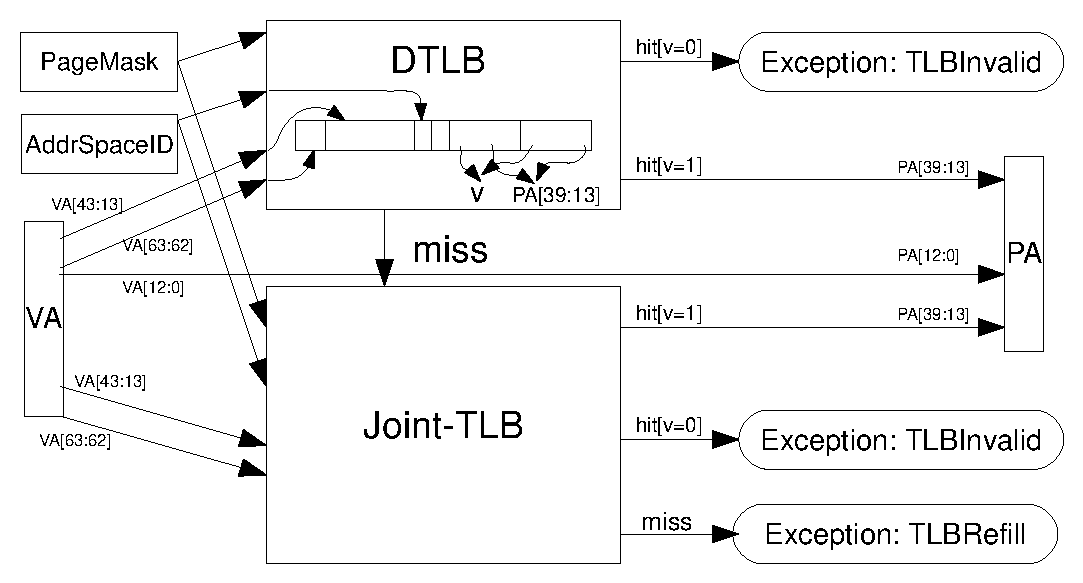
\includegraphics[width=0.8\textwidth]{4.analysis/mips_addrtrans}\\
  \caption{Трансляция адреса в MIPS}\label{fig:mips_address_translation}
\end{figure}


В зависимости от значения виртуального адреса и состояния управляющих регистров
возможны следующие варианты трансляции адреса:
\begin{itemize}
  \item для виртуального адреса трансляция проходит через TLB
(см.рис.~\ref{fig:mips_address_translation});
  \item для виртуального адреса трансляция проходит без таблиц (физический адрес
--- битовая строка --- является результатом битовых операций над виртуальным
адресом --- битовой строкой).
\end{itemize}

Пример модели инструкции LD с рисунка~\ref{fig:mips64_page} приведен в приложении~\ref{sec:xml}.

\section{Генерация тестов для архитектуры PowerPC}

Архитектура PowerPC разработана компанией IBM. Документация по архитектуре
PowerPC представлена в PowerPC Architecture Book (в трех томах)~\cite{PowerPC}. Первый том (PowerPC User Instruction Set Architecture) содержит описания инструкций, которые действительно описываются в виде набора операций над битовыми строками (см.рис.~\ref{fig:ppc_page}.

\begin{figure}
\textbf{Store Halfword Indexed X-form}

sthx RS,RA,RB

\begin{verbatim}
if RA = 0 then b <- 0
else           b <- (RA)
EA <- b + (RB)
MEM(EA, 2) <- (RS)48:63
\end{verbatim}

Let the effective address \texttt{(EA)} be the sum \texttt{(RA|0)+(RB)}. \texttt{(RS)48:63} are stored into the halfword in storage addressed by \texttt{EA}.\\

\textbf{Special Registers Altered:}\\
None
\caption{Пример страницы документации системы команд PowerPC}\label{fig:ppc_page}
\end{figure}

Третий том (PowerPC Operating Environment Architecture) содержит описание подсистемы управления памяти в микропроцессорах PowerPC. Для работы с данными она содержит следующие блоки (количественные характеристики приведены для микропроцессора PowerPC 970FX
~\cite{PowerPC970FXUserManual}):
\begin{itemize}
  \item \emph{кэш-память данных первого уровня (D-Cache-1)}:
        \begin{itemize}
            \item размер: 32 кБ;
            \item поля строк: тэг физического адреса (ключ), данные (данные);
            \item битовая длина номера региона: 7 (наборно-ассоциативная
кэш-память);
            \item количество строк в регионе: 2;
            \item стратегия вытеснения \LRU;
        \end{itemize}
  \item \emph{кэш-память второго уровня (Cache-2)}:
        \begin{itemize}
            \item размер: 512 кБ;
            \item поля строк: тэг физического адреса (ключ), данные (данные);
            \item битовая длина номера региона: 11 (наборно-ассоциативная
кэш~--~память);
            \item количество строк в регионе: 8;
            \item стратегия вытеснения \LRU;
        \end{itemize}
  \item \emph{D-TLB} (кэш таблицы страниц):
        \begin{itemize}
            \item поля строк: номер страницы виртуальной памяти (ключ), номер
фрейма физической памяти (данные);
            \item битовая длина номера региона: 8 (наборно-ассоциативный);
            \item количество строк в регионе: 4;
            \item стратегия вытеснения \LRU;
        \end{itemize}
  \item \emph{сегментные регистры (SLB, Segment Lookaside Buffer)}:
        \begin{itemize}
            \item поля строк: effective segment id (ключ), virtual segment id
(данные), биты K$_s$/K$_p$, V, N, L, C (данные);
            \item битовая длина номера региона: 0 (полностью ассоциативный);
            \item количество строк в регионе: 64;
            \item вытеснение программное;
        \end{itemize}
        используются для получения виртуального адреса по эффективному;
%  \item \emph{буфер непосредственной трансляции адресов (D-ERAT)}:
% НЕТ ЭТОГО БУФЕРА В АРХИТЕКТУРЕ!!! его добавили в самом микропроцессоре
% PPC970FX
%        \begin{itemize}
%            \item поля строк: номер <<эффективной страницы>> (ключ), номер
% фрейма физической памяти (данные), биты (данные);
%            \item битовая длина номера региона: 6 (наборно-ассоциативная
% таблица);
%            \item количество строк в регионе: 2;
%            \item стратегия вытеснения \FIFO;
%        \end{itemize}
\end{itemize}

Кроме того, в оперативной памяти организуется \emph{таблица страниц виртуальной
памяти (PageTable)}. Хотя формально она не является блоком микропроцессора, но
используется при трансляции адреса, то она тоже может быть оформлена в виде
такой таблицы:
    \begin{itemize}
        \item поля строк: номер страницы виртуальной памяти (ключ), номер фрейма
физической памяти (данные);
        \item битовая длина номера региона: 65;
        \item количество строк в регионе: 1;
        \item вытеснение программное;
        \item размер эффективного адреса: 64 бита;
        \item размер виртуального адреса: 65 бит;
        \item размер физического адреса: 42 бита;
    \end{itemize}

На самом деле таблица страниц виртуальной памяти организована в виде сложной
хэш-таблицы, но для тестирования этот момент не важен --- главное, что это
соответствие номеров страниц виртуальной памяти номерам фреймов физической
памяти, причем необязательно представлены все страницы виртуальной памяти.

Другие блоки для обращения в память не используются.

Осталось показать, что трансляция адреса также может быть представлена в виде
отношений на битовых строках и обращениях в таблицы. Обычное выполнение
обращения к памяти в PowerPC следующее:
\begin{enumerate}
    \item аргументы инструкции обращения к памяти формируется \emph{эффективный
адрес} (EA);
    \item заменой номера сегмента из эффективного адреса получается
\emph{виртуальный адрес} (VA);
    \item заменой номера виртуальной страницы в виртуальном адресе на номер
фрейма физической памяти получается \emph{физический адрес} (PA);
    \item по физическому адресу, если нужно, осуществляется обращение в
кэш-память иди, если данных по физическому адресу нет в кэш-памяти, обращение в
оперативную память.
\end{enumerate}

В зависимости от состояния управляющих регистров возможны следующие варианты
трансляции адреса:
\begin{itemize}
  \item real addressing mode (трансляция выключена); физический адрес
вычисляется по эффективному без обращения к каким-либо таблицам;
  \item режим с трансляцией адреса (см. рис.~\ref{fig:ppc_address_translation}).
\end{itemize}

\begin{figure}[h] \center
  \includegraphics[width=\textwidth]{4.analysis/ppc_addrtrans}\\
  \caption{Трансляция адреса в PowerPC}\label{fig:ppc_address_translation}
\end{figure}


\section{Генерация тестов для архитектуры IA-32}

IA-32 --- это архитектура, разрабатываемая компанией Intel. Документация по
архитектуре IA-32 представлена книгой IA-32 Intel® Architecture
Software Developer’s Manual (в пяти томах)~\cite{IA32}. Второй и третий тома \\(Instruction Set Reference) содержат определения инструкций, которые действительно описываются в виде набора операций над битовыми строками (см.рис.~\ref{fig:ia32_page}).

\begin{figure}
\textbf{TEST—Logical Compare}\\

\textbf{Description}\\
Computes the bit-wise logical AND of first operand (source 1 operand) and the second operand
(source 2 operand) and sets the SF, ZF, and PF status flags according to the result. The result is
then discarded.\\

\textbf{Operation}
\begin{verbatim}
TEMP <- SRC1 AND SRC2;
SF <- MSB(TEMP);
IF TEMP = 0
  THEN ZF <- 1;
  ELSE ZF <- 0;
FI:

PF <- BitwiseXNOR(TEMP[0:7]);
CF <- 0;
OF <- 0;
(* AF is undefined *)
\end{verbatim}

\textbf{Flags Affected}\\
The OF and CF flags are set to 0. The SF, ZF, and PF flags are set according to the result (see
the "Operation" section above). The state of the AF flag is undefined.

\caption{Пример страницы документации системы команд архитектуры IA-32}\label{fig:ia32_page}
\end{figure}

Четвертый и пятый тома (System Programming Guide) содержат описание подсистемы управления памяти в
микропроцессорах IA-32. Для работы с данными она содержит следующие блоки
(количественные характеристики приведены для микропроцессора Intel Pentium
Pro~\cite{PentiumPro}) :
\begin{itemize}
  \item \emph{кэш-память данных первого уровня (D-Cache-1)}:
        \begin{itemize}
            \item размер: 8 кБ;
            \item поля строк: тег адреса (ключ), данные (данные);
            \item битовая длина номера региона: 7 (наборно-ассоциативный);
            \item количество строк в регионе: 2;
            \item стратегия вытеснения \LRU;
        \end{itemize}

  \item \emph{кэш-память второго уровня (Cache-2)}:
        \begin{itemize}
            \item размер: в разных версиях 256 кБ, 521 кБ или 1 МБ;
            \item поля строк: тег адреса (ключ), данные (данные);
            \item битовая длина номера региона: от 11 до 13 в разных версиях
(наборно-ассоциативный);
            \item количество строк в регионе: 4;
            \item стратегия вытеснения \LRU;
        \end{itemize}

  \item \emph{TLB (D-TLB)}:
        \begin{itemize}
            \item поля строк: page number (ключ), page base address (данные),
флаги (данные);
            \item битовая длина номера региона: 4 (наборно-ассоциативный);
            \item количество строк в регионе: 4;
            \item стратегия вытеснения \LRU;
        \end{itemize}

  \item \emph{таблица страниц виртуальной памяти (PageTable)}:
    \begin{itemize}
        \item поля строк: page number (ключ), page base address (данные), флаги
(данные);
        \item битовая длина номера региона: 65;
        \item количество строк в регионе: 1;
        \item вытеснение программное;
        \item размер логического адреса: 48 бит;
        \item размер линейного адреса: 32 бит;
        \item размер физического адреса: 32 бита;
    \end{itemize}


  \item \emph{таблица дескрипторов сегментов (SDT)}:
        \begin{itemize}
            \item поля строк: segment selector (ключ), база (данные), флаги
(данные);
            \item битовая длина номера региона: 13;
            \item количество строк в регионе: 1;
            \item вытеснение программное;
        \end{itemize}
\end{itemize}

Другие блоки для обращения в память не используются.

\begin{figure}[h] \center
  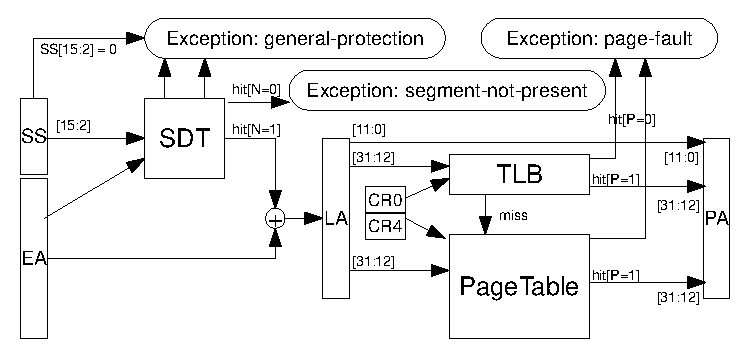
\includegraphics[width=0.8\textwidth]{4.analysis/ia32_addrtrans}\\
  \caption{Трансляция адреса в IA-32}\label{fig:ia32_address_translation}
\end{figure}

Осталось показать, что трансляция адреса также может быть представлена в виде
отношений на битовых строках и обращениях в таблицы. Обычное выполнение
обращения к памяти в IA-32 следующее:
\begin{enumerate}
    \item аргументы инструкции обращения к памяти формируется \emph{логический
адрес} (SS:EA);
    \item заменой номера сегмента из логического адреса получается
\emph{линейный адрес} (LA);
    \item либо линейный адрес трактуется как физический, либо заменой номера
виртуальной страницы в линейном адресе на номер фрейма физической памяти
получается физический адрес (PA);
    \item по физическому адресу, если нужно, осуществляется обращение в
кэш-память иди, если данных по физическому адресу нет в кэш-памяти, обращение в
оперативную память.
\end{enumerate}

В зависимости от состояния управляющих регистров возможны следующие варианты трансляции адреса:
\begin{itemize}
  \item real-address mode (трансляция выключена) --- физический адрес равен линейному, линейный адрес вычисляется по логическому без обращения к каким-либо таблицам;
  \item protected mode --- режим с трансляцией адреса через таблицу страниц (см. рис.~\ref{fig:ia32_address_translation}).
\end{itemize}



\section{Реализация}

Реализация генератора программ состоит из компонентов, представляющих следующие <<деятельности>> (см. рис.~\ref{fig:activities}):
\begin{figure}[h] \center
  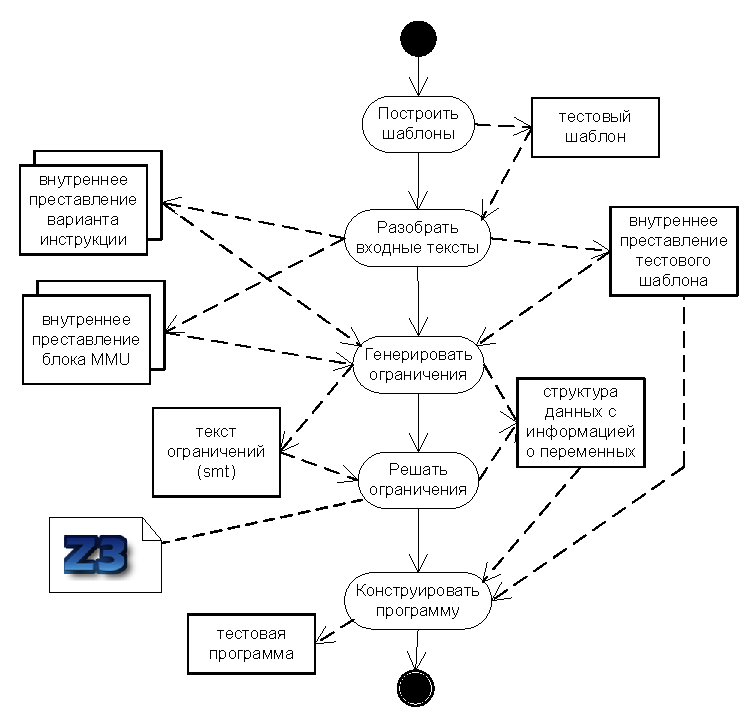
\includegraphics[width=0.7\textwidth]{3.impl/activities1}\\
  \caption{Диаграмма деятельностей по генерации тестовых программ}\label{fig:activities}
\end{figure}
\begin{enumerate}
  \item генерация тестовых шаблонов;
  \item синтаксический анализ исходных текстовых данных; создается внутреннее представление шаблона, моделей блоков, моделей вариантов инструкций для других компонентов;
  \item генерация (текстов) ограничений с использованием описанных в разделах~\ref{sec:constraints_generation_section} и \ref{sec:usefulness_functions} методов (smt~\cite{SMT}); кроме того строится структура, хранящая семантическую информацию о созданных переменных в ограничениях;
  \item обертка решателя ограничений; вызывается внешний решатель ограничений, берется результат его работы, извлекаются из него значения переменных и эти значения прописываются в созданной ранее структуре;
  \item конструирование текстов программ на основе внутреннего представления шаблона и значениях переменных.
\end{enumerate}

Реализация для модельного микропроцессора архитектуры MIPS64~\cite{mips64II} включала следующие компоненты:
\begin{itemize}
  \item генератор тестовых шаблонов внешний --- MicroTESK~\cite{MicroTESK};
  \item решатель ограничений внешний --- Z3~\cite{Z3};
  \item синтаксический анализ моделей, генерация текстов ограничений, обертка решателя ограничений --- компонент <<Генератор ограничений>> на Ruby (порядка 2000 строк);
  \item конструирование тестовых программ --- компонент на Java (порядка 500 строк).
\end{itemize}

Типичный размер модели варианта инструкции --- 100 строк (в представлении на xml). Типичный размер модели блока --- 20 строк (в представлении на xml).

Генератор ограничений практически целиком переносим при смене архитектуры.

\section{Оценка допустимой сложности тестовых\\шаблонов}\label{sec:templates_estimation}

%эксперименты с длинами и временем генерации/процентом успешной
%генерации. Показать, что допустимая длина действительно увеличивается!

Был реализован прототип генератора ограничений для модельного микропроцессора архитектуры
MIPS64~\cite{mips64II}. В качестве решателя ограничений в нем использовался Z3~\cite{Z3}. Был проведен ряд экспериментов. Целью этих экспериментов было исследование допустимой сложности тестовых шаблонов при использовании предлагаемых в диссертации методов (под сложностью понимается
качество шаблона, пропорциональное количеству зависимых данных в нем).

В экспериментах тестовые шаблоны состояли из инструкций загрузки и сохранения
данных в памяти. В каждой инструкции должна была выполняться трансляция адреса
через TLB (с использованием D-TLB) и затем обращение в основную память через
кэш-память первого уровня. Рассматривались все длины тестовых шаблонов от 2 до
16. Для каждой длины рассматривались следующие ассоциативности кэш-памяти --- 2,
4, 8 и 16. При фиксированной длине шаблона и ассоциативности кэш-памяти
случайным образом генерировался тестовый шаблон (более конкретно, зависимости
аргументов инструкций).

Рисунки~\ref{fig:success_experiment} и~\ref{fig:time_experiment} представляют
некоторые средние значения (среднее бралось по всем тестовым шаблоном
фиксированной длины). На рисунке~\ref{fig:success_experiment} отражена доля
шаблонов, для которых был построен тест за время, меньшее чем 60 секунд (если
время превышало 60 секунд, построение теста обрывалось). На
рисунке~\ref{fig:time_experiment} отражено среднее время генерации теста (по
сути, среднее время разрешения ограничений). Более точно, среднее время
продуктивного принятия решения о тестовом шаблоне, т.е. время определения того,
что шаблон является несовместным (для него не может быть теста вовсе) или
совместным с построением теста.

Эксперименты проходили на компьютере AMD Athlon64 3200+ 2ГГц с 1ГБ оперативной
памяти.

\begin{figure}[p] \center
\parbox[t]{\textwidth}{
  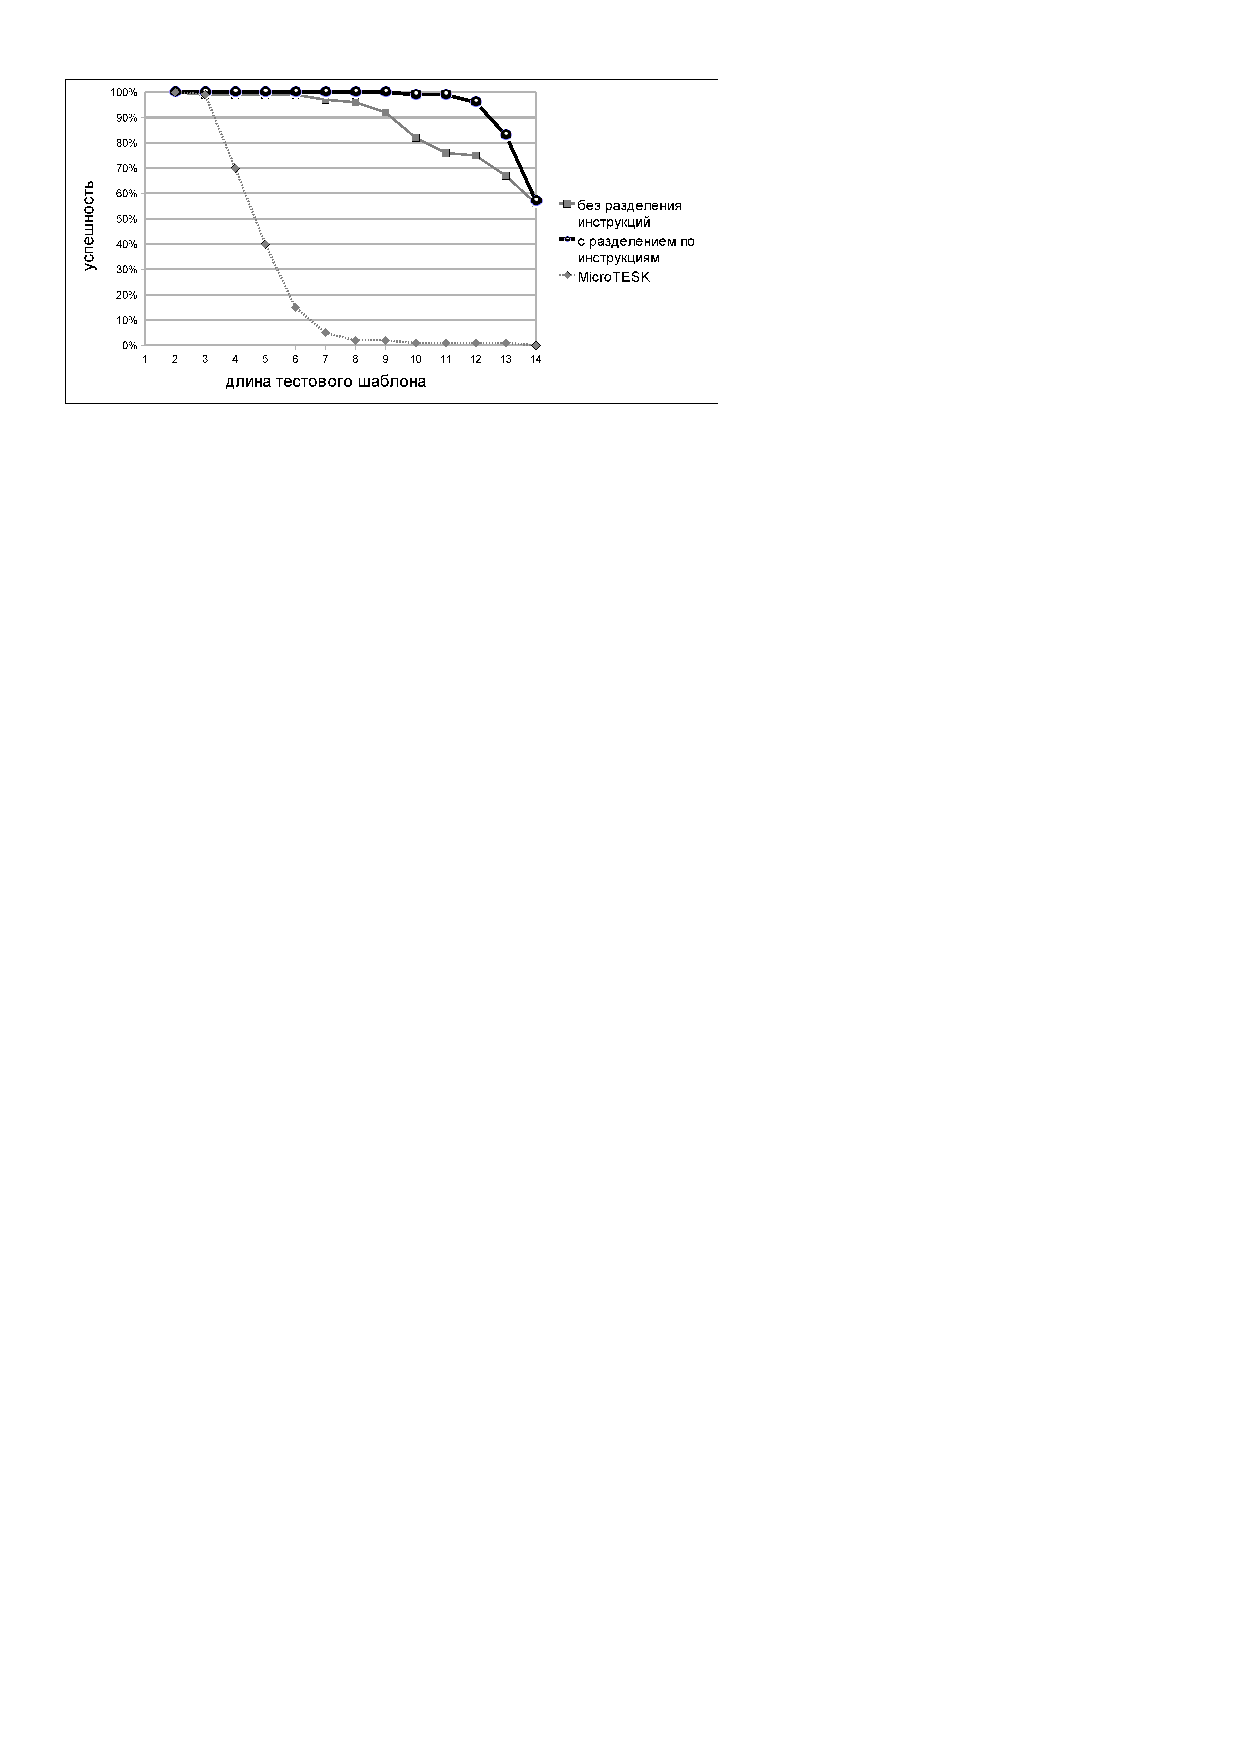
\includegraphics[width=\textwidth]{4.analysis/success_exprmnt}%
\caption{Доля тестовых шаблонов, для которых удалось построить тест за 60с или
определить их несовместность}\label{fig:success_experiment}
}

\vspace{1.5cm}

\parbox[t]{\textwidth}{
  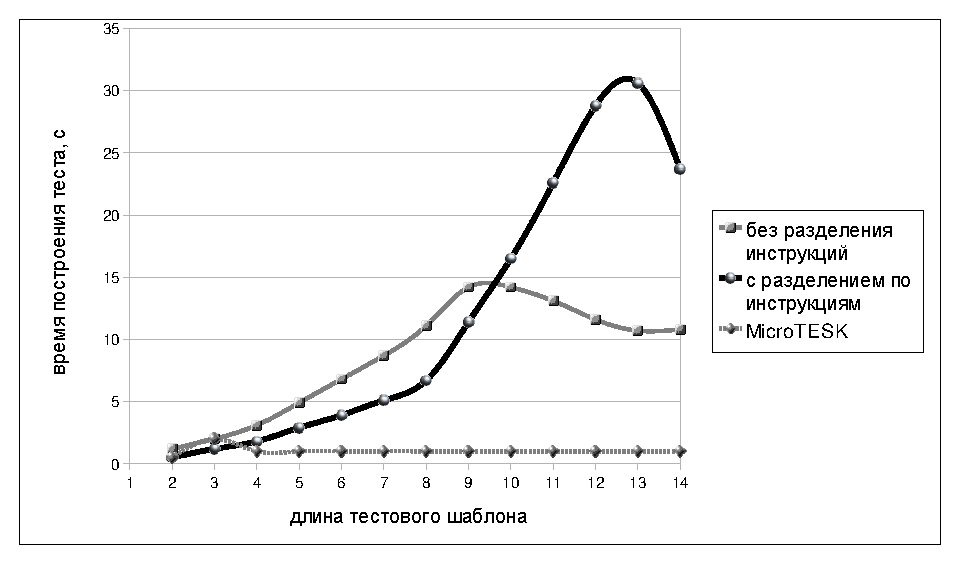
\includegraphics[width=\textwidth]{4.analysis/time_exprmnt}
  \caption{Среднее время продуктивного принятия решения о тестовом
шаблоне}\label{fig:time_experiment}
}
\end{figure}

В первой серии экспериментов (их результаты отражены на рисунках линиями с
квадратиками) генерация ограничений делалась для всего тестового шаблона.
Оказалось, что до некоторой длины шаблона (значит, и теста) (8-9) метод работает
успешно практически для всех тестовых шаблонов (97\%-100\%). При дальнейшем
увеличении длины шаблона начинает уменьшаться доля шаблонов, для которых удается
построить тест (по 5-10\% при увеличении длины теста). Тем самым при длине теста
порядка 14-15 уже для половины шаблонов решатель ограничений не успевает за 60
секунд принять решение и построить тест. В результате анализа использованных в
экспериментах тестовых шаблонов был сделан вывод, что для большинства из них
(60-70\%) тестов не может быть вовсе, так как в этих шаблонах имеются обращения
по одинаковым адресам с кэш-промахами после кэш-попаданий и кэш-промахами после
кэш-промахов (поскольку в результате кэш-промаха данные помещались в кэш-память
и при повторном обращении к ним должно происходить только кэш-попадание, а не
кэш-промах).

Поскольку эта ситуация стала по сути следствием случайного выбора тестовых
шаблонов, то в следующей серии экспериментов перед запуском генерации
ограничений была вставлена процедура, отсеивающая априори несовместные тестовые
шаблоны (т.е. такие, для которых не может существовать тестов вовсе). Кроме того
обращения в кэш-память были поделены на группы на основе одинаковых имен
аргументов и для этих групп генерировались ограничения (грубо говоря, к шаблону
добавлялось требование обращения по разным именам аргументов в разные регионы,
если это не противоречило шаблону). Результаты этой второй серии экспериментов
отражены на рисунках~\ref{fig:success_experiment} и \ref{fig:time_experiment}
линией с кружками. Из них следует, что примененные изменения позволили
дополнительно увеличить на несколько единиц допустимый размер тестового шаблона.

Для каждой пары (длина шаблона, ассоциативность) было сгенерировано 1000
тестовых шаблонов. Насколько можно доверять полученным в экспериментах
результатам на таком количестве тестовых шаблонов? Для ответа на этот вопрос воспользуемся аппаратом теории
вероятностей. Пусть $N$ --- количество испытаний. Одно испытание заключается в
следующем: сначала случайным образом строится тестовый шаблон, затем генерируются
для него ограничения и, наконец, они разрешаются. Испытание заканчивается успешно, если за отведенное время (60с) решатель ограничений построил тест, и неуспешно, если не успел построить.
Обозначим  $\xi_i$, $i = 1, 2, \dots, N$, случайные величины, соответствующие
успешности испытаний. Их областью значений будет множество $\{0, 1\}$. Эти
случайные величины независимы и одинаково распределены (обозначим $p =
\mathsf{P}\{\xi_i = 1\}$). Поэтому применим \emph{закон больших чисел}, согласно
которому $\frac{\sum_{i=1}^N \xi_i}{N} ~ p$ при <<больших>> $N$. Более точно, для любых
положительных $\varepsilon$ и $\delta$ найдется число $N^*$, что для всех $N > N^*$ будет
выполнено $\mathsf{P}\{|\frac{\sum_{i=1}^N \xi_i}{N} - p | \geq \varepsilon\} \leq \delta$. $\varepsilon$ --- это допустимое отклонение в оценке результата экспериментов (т.е. оценке $p$). $\delta$ показывает, насколько можно доверять полученному результату экспериментов. Поскольку $\sum \xi_i$ распределена по биномиальному закону ($\mathsf{P}\{\sum_{i=1}^N \xi_i = m\} = \binom{N}{m} p^m (1{-}p)^{N{-}m}$), то для вероятности отклонения более, чем на $\varepsilon$, справедлива следующая формула: $$\sum_{m = 0}^{(p-\varepsilon)N} \binom{N}{m} p^m (1{-}p)^{N{-}m} + \sum_{m = (p+\varepsilon)N}^N \binom{N}{m} p^m (1{-}p)^{N{-}m} \leq \delta$$ Эта формула позволяет оценить $\delta$ при разных $p$, зная $\varepsilon$ и $N$.

Итак, для каждого $n \in \{2,3\}$ ($n$ --- длина тестового шаблона) было сгенерировано по $B = 1000$ тестовых шаблонов. При этом получилось $p \in [0.9, 1.0]$. Если взять допустимое отклонение от истинного значения $\varepsilon = 0.02$ (2\%) (что вполне допустимо, т.к. отклонение в 2\% не сильно изменит результат эксперимента), то вероятность ошибиться в этом случае была бы не более $\delta = 0.03$, т.е. 3\%, что тоже вполне допустимо. Для $n \in \{4, 5, 6, 7\}$ было сгенерировано по $N = 2000$ тестовых шаблонов (для $w \in \{2,4\}$). Если взять $\varepsilon = 0.02$ (2\%), то для $p \in [0.9, 1.0] \delta = 0.003$, т.е. $0.3\%$, т.е. ошибка в этом случае еще меньше. И, наконец, для $n \in \{8, 9, ..., 14\}$ было сгенерировано по $N = 3000$ тестовых шаблонов, что при $\varepsilon = 0.02$ и $p \in [0.5, 1.0]$ дает $\delta = 0.02$, т.е. всего 2\%. Таким образом, вероятность ошибки в проведенных экспериментах невелика.

Проведенные эксперименты позволяют произвести сравнение с инструментом
MicroTESK~\cite{MicroTESK}. Этот инструмент был успешно применен для построения
тестов по всевозможным тестовым шаблонам из 2-3 инструкций~\cite{vorobyev}. При
увеличении длины тестового шаблона (и, соответственно, сложности) удается
строить тесты для всё меньшего количества шаблонов. Что и отражено на
рисунках~\ref{fig:success_experiment} и \ref{fig:time_experiment} линиями с
ромбами. Напротив, как показывают эксперименты, предложенные методы позволяют
строить тесты по шаблонам из 8-11 инструкций обращения к памяти. Допустимая
длина шаблонов может быть еще больше, если кроме инструкций обращения к памяти в
шаблоне используются и другие инструкции (например, арифметические).

\section{Сравнение с Genesys-Pro}

В прошлом разделе было произведено сравнение с инструментом\\
MicroTESK~\cite{MicroTESK}. В этом разделе будет произведено сравнение с другим
инструментом нацеленной генерации тестов --- Genesys-Pro~\cite{GenesysPro}. Сравнить
по эффективности и провести эксперименты с Genesys-Pro не удается, поскольку
этот инструмент не распространяется за пределы IBM. Однако имеется ряд
публикаций~\cite{GenesysPro2004Innovations, GenesysSolver}, на основе которых удалось сделать некоторое сравнение.

Технологически генерация тестов с использованием Genesys-Pro выглядит следующим
образом:
\begin{enumerate}
    \item подготовить Architectural simulator --- эталонный симулятор
микропроцессора;
    \item подготовить Architectural model --- описание системы команд
тестируемого микропроцессора с указанием для каждой инструкции набора атрибутов
и ограничений значений атрибутов (по сути, описание в виде ограничений
предусловий инструкций и вычисляемым им функций); пример описания инструкции
LoadWord изображен на рисунке~\ref{fig:GenesysProArchitecturalModel}; для
описания трансляции адреса предлагается метод DeepTrans~\cite{DeepTrans} ---
пример изображен на рисунке~\ref{fig:DeepTransExample};
    \item подготовить Test template --- тестовый шаблон; в нем задаются
инструкции теста и интересные для тестирования ситуации исполнения инструкций;
    \item подготовить Testing knowledge --- комплект ограничений на аргументы
инструкций, описывающих ситуации исполнения инструкций из test template;
    \item подготовить или использовать имеющийся решатель ограничений;
    \item запустить Genesys-Pro с подготовленными моделями.
\end{enumerate}
%% я понимаю, что такую последовательность шагов нельзя называть
%% технологической, ибо непоятно
%% 1) как выбирать Testing knowledge - что туда включать, а что нет; наверняка,
%% есть некое понимание того, что хочется протестировать; это понимание
%% должно быть формализовано (модель покрытия) и на его основе уже решать,
%% что включать в Testing knowledge, а что нет;
%% 2) не описано, как анализировать результаты Genesys-Pro: всё ли он сделал или
%% нет, надо ли дорабатывать то, что он генерирует? Надо ли как-то иначе
%% формулировать модели с шагов 1-3 для того, чтобы тесты были построены
%% целиком. И что значит "целиком"? Нет ведь модели покрытия!

\begin{figure}[h] \center
  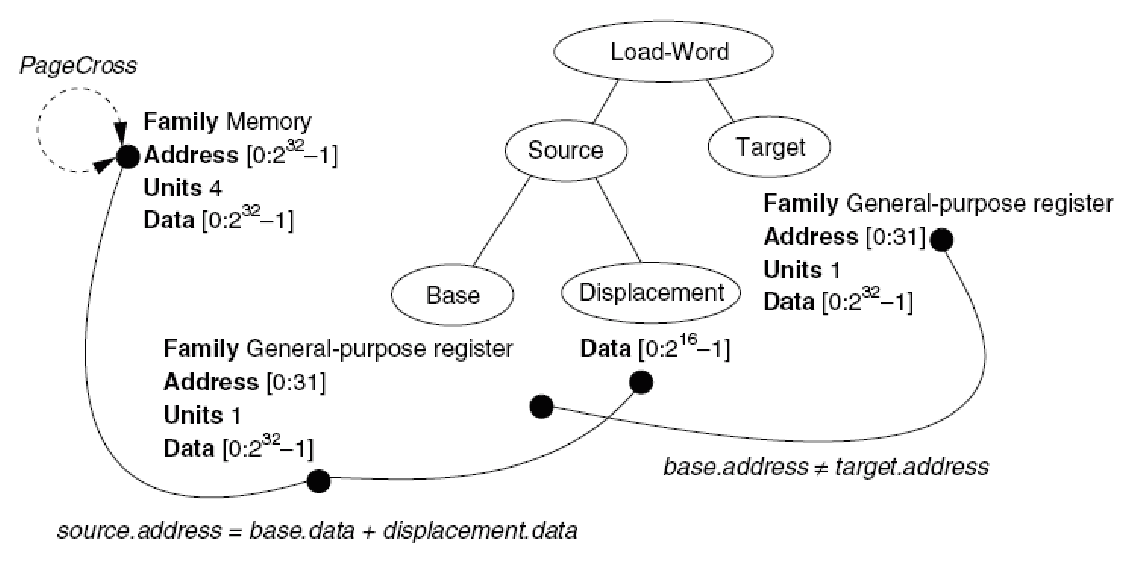
\includegraphics[width=0.8\textwidth]{4.analysis/arch-model}
  \caption{Architectural model для инструкции
LoadWord}\label{fig:GenesysProArchitecturalModel}
\end{figure}

\begin{figure}[h] \center
  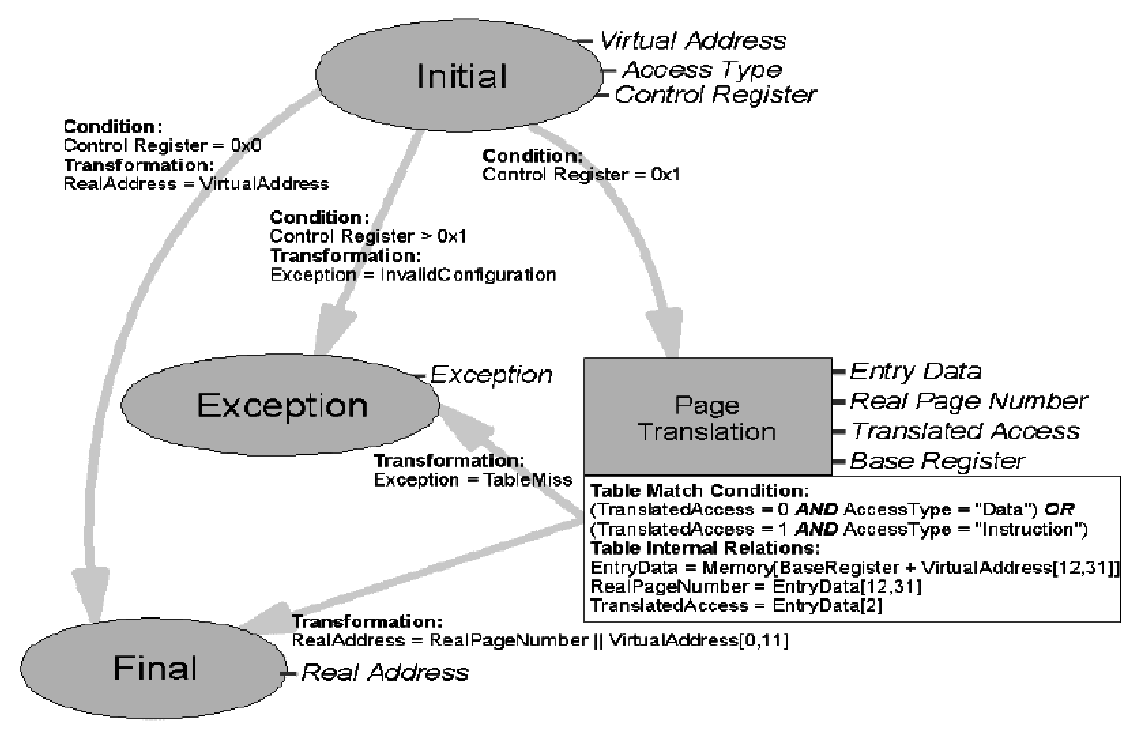
\includegraphics[width=0.8\textwidth]{4.analysis/deeptrans}
  \caption{Пример трансляции адреса в DeepTrans}\label{fig:DeepTransExample}
\end{figure}

\begin{figure}[h] \center
  \includegraphics[width=\textwidth]{4.analysis/g-pro}
  \caption{Genesys-Pro (слева) и предлагаемый в диссертации генератор
(справа)}\label{fig:GenesysProScheme}
\end{figure}

Genesys-Pro работает следующим образом: (см. левую часть
рис.~\ref{fig:GenesysProScheme})
\begin{enumerate}
    \item выбирает очередную инструкцию из Test template, для нее запрашивает
определение из Architectural model и для указанной для нее тестовой ситуации
запрашивает определение из Testing knowledge; кроме того запрашивает текущее
состояние микропроцессора у Architectural simulator;
    \item составляет из этого систему ограничений, передает их для разрешения на
costraint solver и получает ответ;
    \item формирует инструкцию и записывает ее в Test program, а также формирует
часть начального состояния (initial state);
    \item исполняет инструкцию на Architectural simulator, тот ее исполняет.
\end{enumerate}
% т.е. получается, симулятор должен быть каким-то особенным, чтобы уметь
% работать из неполного состояния? (с lazy-значениями 'X') поскольку не
% всё начальное состояние построено перед
% первой инструкций и достраивается в процессе построения теста

\paragraph{Сходства с Genesys-Pro} следующие:
\begin{itemize}
    \item подход, в котором тестовый шаблон и микропроцессор описываются
декларативным образом, и кроме этого есть независимый от них генератор, который
принимает на вход эти описания и строит тест; альтернативным решением могла быть
технология, в которой по модели вручную приходилось бы создавать дополнительные
исполнительные модули, учитывающие особенности модели микропроцессора и
тестового шаблона;
    \item использование ограничений (constraints) для построения тестов;
    \item сходные идеи есть и в методе описания трансляции адресов: Genesys-Pro
предлагает декларативное описание, в котором описываются разные варианты
трансляции с указанием того, как формируются виртуальные/физические адреса, и в
предлагаемом в диссертации подходе описывается формирование адресов; и там, и
там речь идет о \emph{таблицах}, для которых формулируются атрибуты (в том числе
и предикат типа keyMatch).
\end{itemize}

\paragraph{Отличия от Genesys-Pro} следующие:
\begin{itemize}
    \item разные принципы построения ограничений; Genesys-Pro строит тест по
одной инструкции и формулирует ограничения только для одной очередной
инструкции; напротив, в предлагаемом методе ограничения строятся для всего
тестового шаблона целиком;
    \item разные методы построения ограничений; Genesys-Pro знает всё состояние
микропроцессора целиком при формулировании ограничения на очередную инструкцию;
напротив, в предлагаемом методе ограничения состояние микропроцессора неизвестно
вообще; это приводит к ограничениям разной природы;
    \item Genesys-Pro предполагает для инструкции раздельное описание
вычисляемой функции и ограничений на входные данные; в предлагаемом методе эти
описания оформляются вместе;
    \item Genesys-Pro позволяет компактно описать длинные тесты, но важно то,
что эти возможности позволяют описывать целые классы последовательностей
инструкций;
    \item разный способ описания инструкций; Genesys-Pro предлагает делать это в
виде ограничений на атрибуты инструкции, а здесь --- в виде цепочки операторов;
    \item Genesys-Pro рассчитан на подготовку специальных решателей ограничений;
напротив, в предлагаемом методе используются сторонние решатели ограничений и
отдельно подготавливать их не нужно.
\end{itemize}

\paragraph{Преимущества и недостатки по сравнению с Genesys-Pro}:
\begin{itemize}
    \item с помощью Genesys-Pro удается строить очень длинные тесты, но не обязательно эти тесты будут сложными (иметь большое количество зависимых данных);
    \item существует тестовый шаблон, для которого существует тест, но Genesys-Pro его не построит за некоторое время (без, возможно, неописанных в публикациях эвристик), а предлагаемым в диссертации методом тест будет построен; в этом тестовом шаблоне последовательность инструкций должна быть фиксирована; а возможный пример ситуаций в шаблоне такой: в одной из инструкций должны быть вытеснены некоторые специальные данные, которых нет в текущем состоянии из-за неверного выбора данных для предыдущих инструкций;
    \item тем не менее, возможное отсутствие фиксированной цепочки дает Genesys-Pro бонус, поскольку при наличии выбор инструкции может быть успешно сделан с учетом текущего состояния микропроцессора;
    \item Genesys-Pro приходится работать с большими массивами данных (это память, всевозможные кэши и таблицы страниц), эти массивы данных участвуют в ограничениях; поэтому в решателе ограничений приходится разрабатывать методы эффективной работы с ними~\cite{GenesysSolver}; задача построение такого решателя обладает высокой сложностью (как и задача построения эффективного решателя ограничений вообще); кроме того, большая часть такого решателя может оказаться невостребованной при работе с другой моделью микропроцессора, с другим классом тестовых шаблонов --- его придется писать заново; а в предлагаемом методе разрабатывать собственные решатели не нужно.
\end{itemize}

%Genesys-Pro чётко разделяет свойства аргументов
%инструкции и свойства результата инструкции, соотношение между ними
%задается не с помощью ограничений (т.е. не декларативным способом),
%а в виде алгоритма (т.е. императивным способом).
%
%Другой особенностью Genesys-Pro является то, что поддерживаемые им
%тестовые шаблоны зачастую не фиксируют последовательность инструкций
%(это позволяет строить более простые ограничения, потому как
%генерируемая последовательность инструкций может по ходу генерации
%подстраиваться под уже сгенерированные инструкции со
%сгенерированными значениями аргументов, под состояние
%микропроцессора, в которое привели сгенерированные инструкции).
%
%Выразительный язык Genesys-Pro для описания ограничений однако
%содержит такие нетривиальные конструкции, как явное использование
%элементов массивов данных, что требует для разрешения продвинутый
%решатель CSP, в том числе и заточенный под особенности генерации
%тестовых данных для тестовых шаблонов (как минимум такие ограничения
%могут включать битовые операции). Подобный решатель был разработан в
%IBM для инструмента Genesys-Pro~\cite{GenesysSolver}. Однако
%создание такого решателя -- отдельное сложное исследование, которое
%не входило в цели данного исследования. В данной работе было принято
%решение использовать доступные существующие решатели (не обязательно
%CSP) и сосредоточиться на упрощении генерируемых ограничений для
%некоторых частных случаев архитектур.
%
%%\begin{figure}[h]
%%\parbox{0.5\textwidth}{ \centering
%%  \includegraphics[width=0.45\textwidth]{3.impl/genesys-pro}
%%} \vline
%%\parbox{0.5\textwidth}{ \centering
%%  \includegraphics[width=0.45\textwidth]{3.impl/mygen}
%%}
%%\caption{Сравнение с Genesys-Pro}\label{comparison_genesyspro}
%%\end{figure}
%
%В отличие от Genesys-Pro в предлагаемом инструменте описание
%семантики инструкций задается в едином виде -- в виде описаний
%тестовых ситуаций~\cite{my_syrcose_2008, my_isp_2008}. Каждая
%тестовая ситуация описывает не только ограничение на свои аргументы,
%но и результат исполнения инструкции \emph{при данном ограничении на
%аргументы} инструкции декларативным образом. В функции, которую
%реализует инструкция, выделяются отдельные \emph{ветви
%функциональности}, ситуации различного поведения инструкций, каждая
%ветвь функциональности становится отдельной тестовой ситуацией.
%Например, инструкция целочисленного сложения ADD может быть
%исполнена либо точно, либо с возникновением переполнения. Поэтому у
%этой инструкции можно выделить 2 ветви функциональности (точное
%исполнение и исполнение с переполнением), каждая ветвь дает свою
%тестовую ситуацию.

\section{Сравнение с работами Intel}

В ряде публикаций~\cite{MicroFORMAL} описывается инструмент MicroFORMAL, разрабатываемый в Intel. Он используется для некоторых задач формальной верификации разрабатываемых микропроцессоров (в частности, для проверки обратной совместимости). В рамках этой работы требуется описывать поведение микропроцессоров, формализовывать инструкции. Авторы статей упоминают \emph{IRL-представление} микрокода (IRL --- Intermediate Representation Language). Спецификация на IRL описывает функциональность инструкции и побочный эффект (изменение <<внешних>> переменных). Ровно ту же цель преследуют и модели инструкций, предлаагемые в данной работе. Спецификация на IRL представляет собой последовательность операторов (эта же идея используется здесь).

IRL включает в себя управляющие операторы (\texttt{if}, \texttt{goto}), поскольку верификация с использованием спецификаций на IRL нацелена в первую очередь на верификацию потоков управления. В данной работе поток управления не предполагает подобных операторов.

IRL позволяет описывать инструкции обращения к памяти. Однако в нем используется только плоская модель памяти (т.е. память как одномерный массив ячеек) с возможностью обращения <<по индексу>>. Напротив, модели инструкций, предлагаемые в данной работе, позволяют описывать работу с памятью более детально, с указанием успешности обращений в различные блоки подсистемы управления памяти. 


% !Mode:: "TeX:UTF-8"
\chapter*{Заключение}
\addcontentsline{toc}{chapter}{Заключение}

Основные научные и практические результаты, полученные в
диссертационной работе и выносимые на защиту, состоят в следующем:

\Results

%Основные результаты диссертации являются новыми, получены автором самостоятельно.




\pagebreak
\appendix
% % !Mode:: "TeX:UTF-8"
\chapter{Таблицы ограничений}
%\addcontentsline{toc}{chapter}{Приложение А: Таблицы ограничений}

\begin{table}[h] \small
\begin{tabular}{|c|c|c|c|}
\hline  & \centering случай &
\begin{tabular}{c}переменная\\перебора\end{tabular} & система \\
\hline \hline \multirow{10}{*}{\rotatebox{90}{кэш-попадание}} &
\makecell[c{p{0.3\textwidth}}]{тегсет находится в начальном
состоянии буфера, к нему нет обращений до данной инструкции и он всё
ещё не вытеснен} & $\lambda \in L_0$ &
$\left\{\begin{array}{l} x = \lambda\\
x \notin \{x_1, ..., x_n\}\\
\bigwedge\limits_{x_m:\mbox{miss}}\sum\limits_{i=1}^W v_m(\xi_i) +
\sum\limits^{m-1}_{i=1} u_m(x_i) < W
\end{array}\right.
$ \\ \hhline{~|---} & \makecell[c{p{0.3\textwidth}}]{тегсет
находится в начальном состоянии буфера, к нему есть обращение до
данной инструкции и он всё ещё не вытеснен} & $\lambda \in L_0$ &
$\left\{\begin{array}{l} x = \lambda\\
x \in \{x_1, ..., x_n\}\\
\bigwedge\limits_{x_m:\mbox{miss}}\sum\limits^{m-1}_{i=1} u_m(x_i) <
W
\end{array}\right.
$ \\  \hhline{~|---} & \makecell[c{p{0.3\textwidth}}]{тегсет был
внесен одним из кэш-промахов и с того момента не вытеснен} & -- &
$\left\{\begin{array}{l}
x \in [x_1, ..., x_n]_{miss}\\
\bigwedge\limits_{x_m:\mbox{miss}}\sum\limits^{m-1}_{i=1} u_m(x_i) <
W
\end{array}\right.
$ \\ \hline \hline \multirow{20}{*}{\rotatebox{90}{кэш-промах}} &
\makecell[c{p{0.3\textwidth}}]{тегсет встречается впервые} & -- &
$\left\{\begin{array}{l} x \notin L_0\\
x \notin [x_1, ..., x_n]_{miss}\\
\end{array}\right.
$ \\ \hhline{~|---} & \makecell[c{p{0.3\textwidth}}]{тегсет ранее
был внесен одной из инструкций шаблона, затем вытеснен} & -- &
$\left\{\begin{array}{l}
x \in [x_1, ..., x_n]_{miss}\\
\bigvee\limits_{x_m : \mbox{miss}}\sum\limits^{m-1}_{i=1} u_m(x_i) \geqslant W\\
\end{array}\right.$ \\  \hhline{~|---} &
\makecell[c{p{0.3\textwidth}}]{тегсет находился в начальном
состоянии буфера и был вытеснен, к нему не было обращений в шаблоне}
& $\lambda \in L_0$ & $\left\{\begin{array}{l}
x = \lambda\\
x \notin \{x_1, ..., x_n\}\\
\bigvee\limits_{x_m : \mbox{miss}}\sum\limits^W_{i=1} v_m(\xi_i) + \sum\limits^{m-1}_{i=1} u_m(x_i) \geqslant W\\
\end{array}\right.
$ \\ \hhline{~|---} & \makecell[c{p{0.3\textwidth}}]{тегсет
находился в начальном состоянии буфера и был вытеснен, к нему было
обращение в шаблоне после последнего внесения в буфер} & $\lambda
\in L_0$ &
$\left\{\begin{array}{l} x = \lambda\\
x \in \{x_1, ..., x_n\}\\
\bigvee\limits_{x_m : \mbox{miss}}\sum\limits^{m-1}_{i=1} u_m(x_i) \geqslant W\\
\end{array}\right.
$ \\ \hline
\end{tabular}
\caption{Таблица систем уравнений в случае стратегии вытеснения
\PseudoLRU c использованием функций полезности}\label{plru_table}
\end{table}


\begin{landscape}
\begin{table}[p]\small
\begin{tabular}{|c|c|c|c|c|c|}
\hline  & \centering случай &
\begin{tabular}{c}переменная\\перебора\end{tabular} & система &
\begin{tabular}{c}функция полезности\\для кэш-попадания\end{tabular} &
\begin{tabular}{c}функция полезности\\для кэш-промаха\end{tabular} \\
\hline \hline \multirow{10}{*}{\rotatebox{90}{кэш-попадание}} &
\makecell[c{p{0.38\textwidth}}]{тегсет находится в начальном
состоянии буфера, к нему нет обращений до данной инструкции и он всё
ещё не вытеснен} & $\lambda_\delta \in D$ &
$\left\{\begin{array}{l} x = \lambda_\delta\\
x \notin \{x_1, ..., x_n\}\\
\sum\limits^n_{i=1} u(x_i) \leqslant w - \delta
\end{array}\right.
$ &
\begin{tabular}{c}
$x_i \in \{ \lambda_{\delta+1}, ..., \lambda_w\}$\\
$\wedge~x_i \notin \{x_1, ..., x_{i-1}\}$
\end{tabular}
& $R(x_i) = R(x)$
\\ \hhline{~|-----}
& \makecell[c{p{0.38\textwidth}}]{тегсет находится в начальном
состоянии буфера, к нему есть обращение до данной инструкции и он
всё ещё не вытеснен} & $\lambda_\delta \in D$ &
$\left\{\begin{array}{l} x = \lambda_\delta\\
x \in \{x_1, ..., x_n\}\\
\sum\limits^n_{i=1} u(x_i) < w
\end{array}\right.
$ &
\begin{tabular}{c}
$x \notin \{x_i, ..., x_n\}~\wedge$\\
$x_i \in \{ \lambda_{\delta+1}, ..., \lambda_w\}$\\
$\wedge~x_i \notin \{ x_{i+1}, ..., x_n\}$\\
\end{tabular}
&
\begin{tabular}{c}
$x \notin \{x_i, ..., x_n\}$\\
$\wedge~R(x_i) = R(x)$\\
\end{tabular}
\\  \hhline{~|-----}
& \makecell[c{p{0.38\textwidth}}]{тегсет был внесен одним из
кэш-промахов и с того момента не вытеснен} & -- &
$\left\{\begin{array}{l} x \in [x_1, ..., x_n]_{miss}\\
\sum\limits^n_{i=1} u(x_i) < w
\end{array}\right.
$ &
\begin{tabular}{c}
$x \notin \{x_i, ..., x_n\}$\\
$\wedge~R(x_i) = R(x)~\wedge$\\
$x_i \notin \{ x_{i+1}, ..., x_n\}$\\
\end{tabular}
&
\begin{tabular}{c}
$x \notin \{x_i, ..., x_n\}$\\
$\wedge~R(x_i) = R(x)$\\
\end{tabular}
\\ \hline \hline \multirow{15}{*}{\rotatebox{90}{кэш-промах}}
& \makecell[l]{тегсет встречается впервые} & -- &
$\left\{\begin{array}{l} x \notin D\\
x \notin [x_1, ..., x_n]_{miss}\\
\end{array}\right.
$ & -- & -- \\ \hhline{~|-----} &
\makecell[l{p{0.38\textwidth}}]{тегсет ранее был внесен одной из
инструкций шаблона, затем вытеснен} & -- & $\left\{\begin{array}{l}
x \in [x_1, ..., x_n]_{miss}\\
\sum\limits^n_{i=1} u(x_i) \geqslant w\\
\end{array}\right.$ &
\begin{tabular}{c}
$x \notin \{x_i, ..., x_n\}$\\
$\wedge~R(x_i) = R(x)~\wedge$\\
$x_i \notin \{ x_{i+1}, ..., x_n\}$\\
\end{tabular}
&
\begin{tabular}{c}
$x \notin \{x_i, ..., x_n\}$\\
$\wedge~R(x_i) = R(x)$\\
\end{tabular}
\\  \hhline{~|-----} &
\makecell[c{p{0.38\textwidth}}]{тегсет находился в начальном
состоянии буфера и был вытеснен, к нему не было обращений в шаблоне}
& $\lambda_\delta \in D$ &
$\left\{\begin{array}{l} x = \lambda_\delta\\
x \notin \{x_1, ..., x_n\}\\
\sum^n_{i=1} u(x_i) \geqslant w - \delta + 1\\
\end{array}\right.
$ &
\begin{tabular}{c}
$x_i \in\{\lambda_{\delta+1}, ..., \lambda_w\}$\\
$\wedge~x_i \notin \{x_1, ..., x_{i-1}\}$\\
\end{tabular}
&
\begin{tabular}{c}
$R(x_i) = R(x)$\\
\end{tabular}
\\ \hhline{~|-----} &
\makecell[c{p{0.38\textwidth}}]{тегсет находился в начальном
состоянии буфера и был вытеснен, к нему было обращение в шаблоне
после последнего внесения в буфер} & $\lambda_\delta \in D$ &
$\left\{\begin{array}{l} x = \lambda_\delta\\
x \in \{x_1, ..., x_n\}\\
\sum\limits^n_{i=1} u(x_i) \geqslant w\\
\end{array}\right.
$ &
\begin{tabular}{c}
$x \notin \{x_i, ..., x_n\}~\wedge$\\
$x_i \in \{\lambda_{\delta+1}, ..., \lambda_w\}$\\
$\wedge x_i \notin \{ x_{i+1}, ..., x_n\}$\\
\end{tabular}
&
\begin{tabular}{c}
$x \notin \{x_i, ..., x_n\}$\\
$\wedge~R(x_i) = R(x)$\\
\end{tabular}
\\ \hline
\end{tabular}
\caption{Таблица систем уравнений для тестовых ситуаций в \LRU
кэширующих буферах c использованием функций
полезности}\label{hit_miss_table}
\end{table}
\end{landscape}

\begin{landscape}
\begin{table}
\begin{tabular}{|c|c|c|c|c|c|}
\hline  & \centering случай &
\begin{tabular}{c}переменная\\перебора\end{tabular} & система &
\begin{tabular}{c}функция\\полезности\\для кэш-\\попадания\end{tabular} &
\begin{tabular}{c}функция\\полезности\\для кэш-\\промаха\end{tabular} \\
\hline \hline \rotatebox{90}{кэш-попадание} & -- & -- & -- & -- & --
\\ \hline \hline \multirow{15}{*}{\rotatebox{90}{кэш-промах}} &
\makecell[c{p{0.35\textwidth}}]{тегсет встречается впервые} & -- &
$\left\{\begin{array}{l} x \notin D\\
x \notin [x_1, ..., x_n]_{miss}\\
\end{array}\right.
$ & -- & -- \\ \hhline{~|-----} &
\makecell[c{p{0.35\textwidth}}]{тегсет ранее был внесен одной из
инструкций шаблона, затем вытеснен} & -- & $\left\{\begin{array}{l}
x \in [x_1, ..., x_n]_{miss}\\
\left[ \sum\limits^n_{i=1} \right]_{miss} u(x_i) \geqslant w - \delta + 1\\
\end{array}\right.$& -- &
\begin{tabular}{c}
$x \notin \{x_i, ..., x_n\}$\\
$\wedge~R(x_i) = R(x)$\\
\end{tabular}
\\  \hhline{~|-----} &
\makecell[c{p{0.35\textwidth}}]{тегсет находился в начальном
состоянии буфера и был вытеснен, к нему не было обращений в шаблоне}
& $\lambda_\delta \in D$ &
$\left\{\begin{array}{l} x = \lambda_\delta\\
x \notin \{x_1, ..., x_n\}\\
\left[ \sum\limits^n_{i=1} \right]_{miss} u(x_i) \geqslant w - \delta + 1\\
\end{array}\right.$ & -- &
\begin{tabular}{c}
$R(x_i) = R(x)$\\
\end{tabular}
\\ \hhline{~|-----} &
\makecell[c{p{0.35\textwidth}}]{тегсет находился в начальном
состоянии буфера и был вытеснен, к нему было обращение в шаблоне
после последнего внесения в буфер} & $\lambda_\delta \in D$ &
$\left\{\begin{array}{l} x = \lambda_\delta\\
x \in \{x_1, ..., x_n\}\\
\left[ \sum\limits^n_{i=1} \right]_{miss} u(x_i) \geqslant w\\
\end{array}\right.$ & -- &
\begin{tabular}{c}
$x \notin \{x_i, ..., x_n\}$\\
$\wedge~R(x_i) = R(x)$\\
\end{tabular}
\\ \hline
\end{tabular}
\caption{Таблица систем ограничений в случае стратегии вытеснения
\FIFO c использованием функций полезности}\label{fifo_table}
\end{table}
\end{landscape}

\begin{landscape}
\begin{table} \small
\begin{tabular}{|c|c|c|c|c|c|}
\hline  & \centering случай &
\begin{tabular}{c}переменная\\перебора\end{tabular} & система &
\begin{tabular}{c}функция полезности\\для кэш-попадания\end{tabular} &
\begin{tabular}{c}функция полезности\\для кэш-промаха\end{tabular} \\
\hline \hline \multirow{10}{*}{\rotatebox{90}{кэш-попадание}} &
\makecell[c{p{0.38\textwidth}}]{тегсет находится в начальном
состоянии буфера, к нему нет обращений до данной инструкции и он всё
ещё не вытеснен} & $\lambda_\delta \in D$ &
$\left\{\begin{array}{l} x = \lambda_\delta\\
x \notin \{x_1, ..., x_n\}\\
\sum\limits^n_{i=1} u(x_i) \leqslant w - \delta
\end{array}\right.
$ &
\begin{tabular}{c}
$x_i \in \{ \lambda_{\delta+1}, ..., \lambda_\Delta\}$\\
$\wedge~x_i \notin \{x_1, ..., x_{i-1}\}$
\end{tabular}
& $R(x_i) = R(x)$
\\ \hhline{~|-----}
& \makecell[c{p{0.38\textwidth}}]{тегсет находится в начальном
состоянии буфера, к нему есть обращение до данной инструкции и он
всё ещё не вытеснен} & $\lambda_\delta \in D$ &
$\left\{\begin{array}{l} x = \lambda_\delta\\
x \in \{x_1, ..., x_n\}\\
\sum\limits^n_{i=1} u(x_i) < w
\end{array}\right.
$ &
\begin{tabular}{c}
$x \notin \{x_i, ..., x_n\}~\wedge$\\
$x_i \in \{ \lambda_{\delta+1}, ..., \lambda_\Delta\}$\\
$\wedge~x_i \notin \{ x_{i+1}, ..., x_n\}$\\
\end{tabular}
&
\begin{tabular}{c}
$x \notin \{x_i, ..., x_n\}$\\
$\wedge~R(x_i) = R(x)$\\
\end{tabular}
\\  \hhline{~|-----}
& \makecell[c{p{0.38\textwidth}}]{тегсет был внесен одним из
кэш-промахов и с того момента не вытеснен} & -- &
$\left\{\begin{array}{l} x \in [x_1, ..., x_n]_{miss}\\
\sum\limits^n_{i=1} u(x_i) < w
\end{array}\right.
$ &
\begin{tabular}{c}
$x \notin \{x_i, ..., x_n\}$\\
$\wedge~R(x_i) = R(x)~\wedge$\\
$x_i \notin \{ x_{i+1}, ..., x_n\}$\\
\end{tabular}
&
\begin{tabular}{c}
$x \notin \{x_i, ..., x_n\}$\\
$\wedge~R(x_i) = R(x)$\\
\end{tabular}
\\ \hline \hline \multirow{20}{*}{\rotatebox{90}{кэш-промах}}
& \makecell[c{p{0.38\textwidth}}]{тегсет встречается впервые} & -- &
$\left\{\begin{array}{l} x \notin D\\
x \notin [x_1, ..., x_n]_{miss}\\
\end{array}\right.
$ & -- & -- \\ \hhline{~|-----} &
\makecell[c{p{0.38\textwidth}}]{тегсет ранее был внесен одной из
инструкций шаблона, затем вытеснен} & -- &
$\left\{\begin{array}{l} x \in [x_1, ..., x_n]_{miss}\\
\sum\limits^n_{i=1} u(x_i) \geqslant w\\
\end{array}\right.
$ &
\begin{tabular}{c}
$x \notin \{x_i, ..., x_n\}$\\
$\wedge~R(x_i) = R(x)~\wedge$\\
$x_i \notin \{ x_{i+1}, ..., x_n\}$\\
\end{tabular}
&
\begin{tabular}{c}
$x \notin \{x_i, ..., x_n\}$\\
$\wedge~R(x_i) = R(x)$\\
\end{tabular}
\\  \hhline{~|-----} &
\makecell[c{p{0.38\textwidth}}]{тегсет находился в начальном
состоянии буфера и был вытеснен, к нему не было обращений в шаблоне}
& $\lambda_\delta \in D$ &
$\left\{\begin{array}{l} x = \lambda_\delta\\
x \notin \{x_1, ..., x_n\}\\
\sum\limits^n_{i=1} u(x_i) \geqslant w - \delta + 1\\
\end{array}\right.
$ &
\begin{tabular}{c}
$x_i \in\{\lambda_{\delta+1}, ..., \lambda_\Delta\}$\\
$\wedge~x_i \notin \{x_1, ..., x_{i-1}\}$\\
\end{tabular}
&
\begin{tabular}{c}
$R(x_i) = R(x)$\\
\end{tabular}
\\ \hhline{~|-----} &
\makecell[c{p{0.38\textwidth}}]{тегсет находился в начальном
состоянии буфера и был вытеснен, к нему было обращение в шаблоне
после последнего внесения в буфер} & $\lambda_\delta \in D$ &
$\left\{\begin{array}{l} x = \lambda_\delta\\
x \in \{x_1, ..., x_n\}\\
\sum\limits^n_{i=1} u(x_i) \geqslant w\\
\end{array}\right.
$ &
\begin{tabular}{c}
$x \notin \{x_i, ..., x_n\}~\wedge$\\
$x_i \in \{\lambda_{\delta+1}, ..., \lambda_\Delta\}$\\
$\wedge~x_i \notin \{ x_{i+1}, ..., x_n\}$\\
\end{tabular}
&
\begin{tabular}{c}
$x \notin \{x_i, ..., x_n\}$\\
$\wedge~R(x_i) = R(x)$\\
\end{tabular}
\\ \hline
\end{tabular}
\caption{Таблица систем уравнений для тестовых ситуаций в \LRU
кэширующем буфере c <<грязными>> ячейками в начальном состоянии,
использующих функции полезности}\label{dirty_hit_miss_table}
\end{table}
\end{landscape}

%TODO!!! % !Mode:: "TeX:UTF-8"
\chapter{Доказательства теорем и лемм}\label{sec:proofs}
%\addcontentsline{toc}{chapter}{Приложение А: Таблицы ограничений}

\begin{lemma}\label{QuantorElimination}
Для любых неотрицательных чисел $x$, $y$ и $N$ таких, что $0 \leqslant x, y < 2^N$, справедливо следующее (сравнения беззнаковые):
$$( \exists k \in \mathds{N} : x < 2^k \leqslant y ) \Leftrightarrow (y > x ~\wedge~ x \oplus y > x)$$
\end{lemma}
\begin{proof}
  // TODO
\end{proof}

\theoremtext{\ref{mirror_fullness_none}}{\FullnessMirrorNone}
\begin{proof}
  Особо подчеркну сначала, что в формулировке теоремы $n$ --- количество обращений к таблице в тестовом шаблоне. А в алгоритме построения ограничений $n$ --- количество \textbf{успешных} обращений к таблице в тестовом шаблоне. Чтобы согласовать обозначения, будем далее придерживаться обозначений из алгоритма: ключи в регионах с успешными обращениями обозначать как $k_i$, $R_i$ для $i = 1, 2, ..., n$, а ключа в регионах с неуспешными обращениями обозначать как $k'_j$, $R'_j$ для $j = 1, 2, ..., n'$ ($n$ в формулировке теоремы есть новое $n$ + $n'$).

  Обозначим $L$ --- состояние таблицы перед тестовым шаблоном. Тогда согласно посылке в условии теоремы для каждого допустимого $i$ выполнено: $(k_i || R_i) \in L$ --- и для каждого допустимого $j$ выполнено: $(k'_j || R'_j) \notin L$. Для всех инструкций состояние таблицы одно и то же, поскольку стратегия вытеснения есть \texttt{none} (промах лишь фиксируется, но не <<исправляется>>). Тем самым. $L \supseteq \{ (k_1||R_1), ..., (k_n||R_n) \}$. Отсюда следует, что для каждого допустимого $j$ $(k'_j||R'_j) \notin \{ (k_1||R_1), ..., (k_n||R_n) \}$.

  Кроме того, поскольку $L$ --- состояние таблицы перед тестовым шаблоном, то количество ключей в каждом регионе, которое может находиться в $L$ равно $w$ (по определению $w$). Но поскольку $L \supseteq \{ (k_1||R_1), ..., (k_n||R_n) \}$, то количество различных ключей в каждом регионе в последовательности $(k_i, R_i)$ не может быть больше $w$. Осталось показать, что это количество выражается формулой, представленной в алгоритме. Действительно, для получения количества различных ключей в том же регионе достаточно просматривать все ключи с начала и отсчитывать те из них, что встречаются впервые, т.е. не встречаются среди предыдущих ключей, что и выражено в формуле.

  Итак, если для щаблона в заданном начальном состоянии есть какая-нибудь последовательность ключей в регионах, то система ограничений будет совместна, поскольку на этих же ключах и регионах выполнены ограничения, генерируемые согласно алгоритму.
\end{proof}

\theoremtext{\ref{mirror_fullness}}{\FullnessMirror}
\begin{proof}
Докажем даже более сильное утверждение (из него очевидно будет следовать требуемое в теореме): есть начальное состояние таблицы $L_0$, для него существуют такие $k_1, k_2, ..., k_n$, $R_1, R_2, ..., R_n$, что выполнены все $S_i$ и $P$; спрашивается, будут ли существовать такие $t_1, t_2, ..., t_m$, $r_1, r_2, ..., r_m$, что составленные ограничения (для тех же $k_1, k_2, ..., k_n$, $R_1$, $R_2$, ..., $R_n$) будут выполнены. Весь вопрос в том, как выбрать $t_1, t_2, ..., t_m$, $r_1, r_2, ..., r_m$. Доказательство можно разделить на две части: в первой будет предложен способ выбора $t_1, t_2, ..., t_m$, $r_1, r_2, ..., r_m$, а во второй будет показано, что на них выполняются ограничения.

\paragraph{выбор инициализирующей последовательности} предлагается делать\\следующим образом. Она будет состоять из подпоследовательностей $s_R$ для каждого $R$ из \textbf{множества} $\{R_1, R_2, ..., R_n\}$. Далее рассматривается построение такой подпоследовательности для произвольного $R$. Выберем из $L_0$ ключи, хранящиеся в регионе $R$, ровно в том порядке, в каком они там находятся (речь идет о порядке в смысле перестановок в таблицах вытеснения). Обозначим эту последовательность $V \equiv \langle v_1, v_2, ..., v_q \rangle$. Далее, удалим из последовательности $k_1, k_2, ..., k_n$ те ключи, чьи регионы не равны $R$, и те, которые присутствуют в последовательности $v_1, v_2, ..., v_q$. Обозначим получившуюся последовательность $U \equiv \langle u_1, u_2, ..., u_p\rangle$. Если $p < w$, то выберем $p{-}w$ произвольных ключей, не встречающихся в последовательностях $U$ и $V$. Обозначим эту последовательность $Z$. Тогда $s_R$ будет являться конкатенацией последовательностей $Z$, $U$ и $V$ (именно в этом порядке). Порядок конкатенации последовательностей $s_R$ произвольный. Последовательность $r_1, r_2, ..., r_m$ выбирается в соответствии с выбором последовательности конкатенации $s_R$.

\paragraph{выполнение системы ограничений} По построению все $(t_1||r_1)$, $(t_2||r_2)$, ..., $(t_m||r_m)$ разные. Кроме того, поскольку на $(k_i, R_i)$ выполнены все условия в тестовом шаблоне, то для них выполнено условие количества различных пар (ключ, регион) в каждом регионе для каждой инструкции. Далее, поскольку последовательность $(t_i, r_i)$ оканчивается последовательностью, дублирующей $L_0$ и стратегия вытеснения является существенно вытесняющей, то после таких инициализирующих обращений состояние таблиц станет точно таким же, каким оно было до инициализирующих обращений. Это значит, что для $(k_i, R_i)$ выполнены ограничения <<быть вытесненным>> (они и есть $S_i$). И поскольку последовательность $(t_1, r_1)$, $(t_2, r_2)$, .., $(t_m, r_m)$ содержит все $(k_1, R_1)$, ..., $(k_n, R_n)$, то выполнены ограничения\\$(k_i||R_i) \in \{(t_1||r_1), (t_2||r_2), ..., (t_m||r_m), (k_1||R_1), (k_2||R_2), ..., (k_{i-1}||R_{i-1})\}$.
\end{proof}

\begin{lemma}\label{PseudoLRUNolDisplacing}
Рассматривается последовательность промахов при стратегии вытеснения \PseudoLRU. Тогда в результате $w{-}1$ промаха строка региона на позиции 0 не будет вытеснена.
\end{lemma}
\begin{proof}
    Доказательство для лучшей читабельности приведено для случая $w = 8$, хотя всё аналогичное переносится на случай произвольного $w = 2^W$.

    Последняя строка таблицы вытеснения для \PseudoLRU имеет вид:\\$(m~6~4~5~0~1~2~3)$. Если разложить каждую позицию в битовую строку, то эту же перестановку можно задать следующим образом:
    \begin{itemize}
        \item элемент с позиции $x \in \{\bigl(\begin{smallmatrix}0\\0\\0
\end{smallmatrix}\bigr), \bigl(\begin{smallmatrix}0\\0\\1
\end{smallmatrix}\bigr), \bigl(\begin{smallmatrix}0\\1\\0
\end{smallmatrix}\bigr), \bigl(\begin{smallmatrix}0\\1\\1
\end{smallmatrix}\bigr)\}$ перемещается на позицию $x \oplus \bigl(\begin{smallmatrix}1\\0\\0
\end{smallmatrix}\bigr)$;
        \item элемент с позиции $x \in \{\bigl(\begin{smallmatrix}1\\0\\0
\end{smallmatrix}\bigr), \bigl(\begin{smallmatrix}1\\0\\1
\end{smallmatrix}\bigr)\}$ перемещается на позицию $x \oplus \bigl(\begin{smallmatrix}1\\1\\0
\end{smallmatrix}\bigr)$;
        \item элемент с позиции $x \in \{\bigl(\begin{smallmatrix}1\\1\\0
\end{smallmatrix}\bigr)\}$ перемещается на позицию $x \oplus \bigl(\begin{smallmatrix}1\\1\\1
\end{smallmatrix}\bigr)$;
        \item $m$ помещается на позицию 0.
\end{itemize}

Сокращая обозначения, перефразируем это:
\begin{itemize}
    \item элемент с позиции $x = \bigl(\begin{smallmatrix}0\\X\\X\end{smallmatrix}\bigr)$ перемещается на позицию $x \oplus \bigl(\begin{smallmatrix}1\\0\\0 \end{smallmatrix}\bigr)$;
    \item элемент с позиции $x = \bigl(\begin{smallmatrix}1\\0\\X\end{smallmatrix}\bigr)$ перемещается на позицию $x \oplus \bigl(\begin{smallmatrix}1\\1\\0\end{smallmatrix}\bigr)$;
    \item элемент с позиции $x = \bigl(\begin{smallmatrix}1\\1\\0\end{smallmatrix}\bigr)$ перемещается на позицию $x \oplus \bigl(\begin{smallmatrix}1\\1\\1\end{smallmatrix}\bigr)$;
    \item $m$ помещается на позицию 0.
\end{itemize}

Перевернем каждый столбец. Получится следующий набор правил перемещения в результате промаха:
\begin{itemize}
    \item элемент с позиции $x = \bigl(\begin{smallmatrix}X\\X\\0\end{smallmatrix}\bigr)$ перемещается на позицию $x \oplus \bigl(\begin{smallmatrix}0\\0\\1 \end{smallmatrix}\bigr)$;
    \item элемент с позиции $x = \bigl(\begin{smallmatrix}X\\0\\1\end{smallmatrix}\bigr)$ перемещается на позицию $x \oplus \bigl(\begin{smallmatrix}0\\1\\1\end{smallmatrix}\bigr)$;
    \item элемент с позиции $x = \bigl(\begin{smallmatrix}0\\1\\1\end{smallmatrix}\bigr)$ перемещается на позицию $x \oplus \bigl(\begin{smallmatrix}1\\1\\1\end{smallmatrix}\bigr)$;
    \item $m$ помещается на позицию 0.
\end{itemize}

Под действием этих правил происходят $w{-}1$ перемещений с <<перевернутой>> позиции $\bigl(\begin{smallmatrix}0\\0\\0\end{smallmatrix}\bigr)$. Покажем, что это перемещение имеет очень простой вид: 0, 1, 2, ... . Докажем по индукции. База очевидна: позиция изначально равна 0. Индуктивный переход. За позицией $2k$ будет следовать позиция $2k+1$ под действием первого правила. За позицией $2k+1$ будет следовать позиция $2k+2$ под действием остальных правил (0 и последовательность единичных битов инвертируется, что и есть прибавление единицы).

А если перемещение имеет такой вид, то за $w{-}1$ перемещение ни одна из <<перевернутых>> позиций (а, значит, и просто позиций) не равна $w{-}1$ (0, 1, 2, ..., $w{-}2$). А позиция $w{-}1$ --- это и есть позиция вытеснения согласно последней строке таблицы вытеснения для \PseudoLRU.
\end{proof}

\theoremtext{\ref{thm:PseudoLRU_essential}}{\PseudoLRUEssential}
\begin{proof}
    Из леммы~\ref{PseudoLRUNolDisplacing} следует, что первый внесенный в результате промаха $m$ не будет вытеснен после $w{-}1$ промахов. Однако при каждом промахе какие-то элементы вытесняются. Вносимые на каждом промахе $m$ проходят ту же <<траекторию>>, что и первый. Поэтому к ним снова применима лемма~\ref{PseudoLRUNolDisplacing}. Тем самым после $w$ промахов в регионе будет $w$ штук $m$. Но больше, чем $w$, и не может быть, поскольку это количество строк в регионе. Значит, после $w$ промахов весь регион будет состоять лишь из одних $m$.
\end{proof}

\theoremtext{\ref{thm_mirror_lenth_lru}}{\UpperBoundLRUMirror}
\begin{proof}
  Так же, как это было сделано при доказательстве
  теоремы~\ref{mirror_fullness}, разделим все $k_1, k_2, ..., k_n$
  по регионам. Для каждого задействованного региона составим свою
  инициализирующую последовательность (обозначим ее длину $m_i$
  для $i$'го задействованного региона) и сконкатенируем эти
  последовательности для получения искомой инициализирующей последовательности
   для всего тестового шаблона.
  Подпоследовательность последовательности $k_1, k_2, ..., k_n$,
  соответствующая одному региону, обозначим $y_1, y_2, ...,
  y_{n_i}$.

  Докажем, что $$m_i = M_i + w$$ где $M_i$ -- количество
  элементов последовательности $y_1, y_2, ..., y_{n_i}$, которые дают
  промахи при первых обращениях к ним. Тогда для всего тестового
  шаблона $m = \sum\limits_i m_i = \sum\limits_i M_i + \sum\limits_i w =
  M + w \cdot r$, где $r$ -- количество регионов, задействованных в
  $k_1, k_2, ..., k_n$. Очевидно, что $r \leqslant n$, тем самым это
  приводит к искомой оценке $m \leqslant M + n \cdot w$. Осталось
  доказать формулу для $m_i$.

  Укажем способ построения ключей инициализирующей последовательности. Выберем из $y_1, y_2, ..., y_{n_i}$ подпоследовательность,
  состоящую из тех ключей, которые дают промах и встречаются
  впервые. Обозначим их как $\mu \equiv \mu_1, \mu_2, ..., \mu_{MM_i}$. Они будут первыми ключами в   инициализирующей последовательности. Далее выберем из $y_1, y_2, ..., y_{n_i}$
  все ключи, при обращении к которым происходят попадания.
  Обозначим их как $\eta \equiv \eta_1, \eta_2, ..., \eta_{HH_i}$. Если $MM_i > 0$ и $MM_i +
  HH_i < w + 1$, выберем произвольные различные числа-ключи $\nu \equiv \nu_1, \nu_2,
  ..., \nu_{NN_i}$, которые не встречаются в $y_1, y_2, ..., y_{n_i}$. Итак, инициализирующая последовательность (для данного региона!) представляет собой конкатенацию последовательностей $\mu$, $\eta$ и $\nu$ (в этом порядке).

  Покажем, что такая инициализирующая последовательность удовлетворяет системе ограничений. Все ключи из тестового шаблона, при обращении к которым происходят попадания, встречаются в
  этой последовательности. Это следует из того, что первые такие ключи мы поместили явно (в конец последовательности), а дальнейшие ключи не могут встречаться впервые в тестовом шаблоне, в противном случае они были бы вытеснены до того, как должно быть попадание. Очевидно, что эти первые ключи не вытеснены, поскольку они помещены в конец инициализирующей последовательности. Все ключи, при обращении к которыми происходят промахи, тоже встречаются в этой последовательности (мы их туда поместили явно). При этом поскольку от своего промаха они отделены не менее $w+1$ инструкцией с разными ключами, то к моменту промаха они будут
  вытеснены (для первой инструкции это очевидно по построению, а
  для остальных следует из леммы~\ref{includedranges} о невложенных диапазонах вытеснения).

  Длина инициализирующей последовательности для шаблона без промахов (при $MM_i$ = 0) равна количеству ключей в $y_1, y_2, ..., y_{n_i}$, при обращении к
  которым происходят попадания. Их не более чем $w$,
  т.к. последовательность из попаданий может задать лишь часть
  или целиком весь регион. При $MM_i > 0$ длина последовательности
  есть сумма из $M_i$ (поскольку туда включаются все ключи $y_1, y_2,
  ..., y_{n_i}$, при обращении к которым происходят промахи) и
  $w$ (поскольку в инициализирующую последовательность добавляются фиктивные ключи и ключи, при обращении к которым происходят попадания). В обоих случах $m_i = M_i + w$.
\end{proof}

\theoremtext{\ref{thm_pseudoLRU_invariant}}{\PseudoLRUInvariant}
\begin{proof}
  Пусть происходит обращение с позицией $j = (j_1~j_2~\dots~j_W)$.
  Тогда согласно каноническому определению \PseudoLRU будет
  произведены следующие изменения: $B_{(1)} := j_1; B_{(1~j_1)} :=
  j_2; \dots B_{(1~j_1~j_2~\dots~j_{W-1})} := j_W$. Однако только
  часть этих изменений повлияет на
  $(\alpha_1~\alpha_2~\dots~\alpha_W)$, $\alpha_1 = B_{(1)}^{\neg
  i_1}, \alpha_2 = B_{(1~i_1)}^{\neg i_2}, \dots, \alpha_W =
  B_{(1~i_1~i_2~\dots~i_{W-1})}^{\neg i_W}$. А именно влияние будет
  на те элементы вектора, у которых совпадают индексы с изменяемыми
  элементами согласно каноническому определению. Иными словами,
  изменение $B_{(1~j_1~j_2~\dots~j_k)}$ будет влиять на
  $B_{(1~i_1~i_2~\dots~i_m)}$ тогда и только тогда, когда
  $(1~j_1~j_2~\dots~j_k) = (1~i_1~i_2~\dots~i_m)$. Докажем, что при
  этом $k = m$. Действительно, если $k > m$, то
  $(1~j_1~j_2~\dots~j_k) \geqslant 2^k$, а $(1~i_1~i_2~\dots~i_m) <
  2^{m+1} \leqslant 2^k$, что исключает равенство этих чисел.
  Аналогично доказывается невозможность случая $k < m$.

  Условие $(1~j_1~j_2~\dots~j_k) = (1~i_1~i_2~\dots~i_k)$
  эквивалентно условию $(j_1~j_2~\dots~j_k)$ $\oplus~(i_1~i_2~\dots~i_k) =
  0$. Переходя к полным векторам, это условие записывается в виде $(j_1~j_2~\dots~j_W) \oplus
  (i_1~i_2~\dots~i_W) < 2^{W-k+1}$. Или, переходя от векторов к
  числам, $i \oplus j < 2^{W-k+1}$.

  При этом изменение элементов вектора
  ($\alpha_1~\alpha_2~\dots~\alpha_W$) будет происходить следующим
  образом (используется определение степени через сложение по модулю
  2: $x^y \equiv x \oplus y \oplus 1$): $\alpha_k :=
  (B_{(1~j_1~j_2~\dots~j_{k-1})})^{\neg i_k} =
  (B_{(1~j_1~j_2~\dots~j_{k-1})}) \oplus (\neg i_k) \oplus 1 =
  B_{(1~j_1~j_2~\dots~j_{k-1})} \oplus i_k = j_k \oplus i_k$. Так
  как $(j_1~j_2~\dots~j_{k-1}) = (i_1~i_2~\dots~i_{k-1})$, то
  $(j_1~j_2~\dots~j_{k-2}) = (i_1~i_2~\dots~i_{k-2})$ и $i_{k-1} =
  j_{k-1}$. В таком случае изменяется и $\alpha_{k-1}$, причем
  $\alpha_{k-1} := i_{k-1} \oplus j_{k-1} = 0$. Аналогично
  рассуждая, получим, что $\alpha_{k-2} := 0,~\dots~\alpha_1 := 0$.
  Иными словами, возможно даже вычислить изменения предыдущих
  элементов -- всем им присваивается значение 0. Найдется такой $p$,
  что $i_1 = j_1~\wedge~i_2 = j_2~\wedge~i_{p-1} =
  j_{p-1}~\wedge~i_p \neq j_p$. В этом случае изменяется
  $\alpha_p$ следующим образом: $\alpha_p := i_p \oplus j_p = 1$.
  Или записывая это условие с использованием чисел $i$ и $j$: $2^{W-p} \leqslant i
  \oplus j < 2^{W-p+1}$.

  Таким образом, получаем, что для $i \oplus j \in
  [\frac{w}{2^k},~\frac{w}{2^{k-1}})$ будет произведены следующие
  присваивания: $\alpha_k := 1,~\alpha_{k-1} := 0,~\alpha_{k-2} :=
  0,~\dots~\alpha_1 := 0$, остальные элементы не будут изменены. Для
  $i \oplus j = 0$, т.е. $i = j$ все элементы $\alpha_k := i_k \oplus
  j_k = 0$. Причем изменение определяется только суммой по модулю 2
  чисел $i$ и $j$, что и является относительной позицией $j$
  относительно $i$.

  Осталось разобраться с ветвью вытесняемого ключа. Это будет такая
  позиция $i = (i_1~i_2~\dots~i_W)$, для которой справедливы
  уравнения $i_1 = \neg B_{k_1}~\wedge~i_2 = \neg
  B_{k_2}~\wedge~\dots~\wedge~i_W = \neg B_{k_W}$, где $k_1 = (1)$,
  $k_2 = (1~\neg B_{k_1})$, ..., $k_W = (1~\neg B_{k_1}~\neg
  B_{k_2}~\dots\\\neg B_{k_{W-1}})$. Используя уравнения для
  элементов $i$, можно переписать уравнения для элементов $k$
  следующим образом: $k_1 = (1)$,
  $k_2 = (1~i_1)$, ..., $k_W = (1~i_1~i_2~\dots~i_{W-1})$. Таким
  образом, элементы ветви вытесняемого ключа будут вычисляться
  следующим образом: $\alpha_m \equiv B_{(1~i_1~i_2~\dots~i_{m-1})}
  \oplus i_m \equiv B_{k_m} \oplus i_m \equiv \neg i_m \oplus i_m
  \equiv 1$. Иными словами, ветвь вытесняемого ключа состоит только
  из единиц.
\end{proof}


\pagebreak
%%%%\bibliographystyle{plain}
%%%%\bibliographystyle{gost71u}
\addcontentsline{toc}{chapter}{Литература}
\bibliographystyle{gost780s}
\bibliography{thesis}

%% привести оформление в соответствие с требованием: что-то всё время пропадает!

%%! добавить \cite{Pex}, \cite{symbolic_execution}

%%! вписать название препринта и номер тома

\end{document}
